\documentclass[draft, final]{report}
\usepackage[T1]{fontenc}
\usepackage[english]{babel}
\usepackage{enumitem}
\usepackage{amssymb}
\usepackage{textcomp}
\usepackage[utf8]{inputenc}
\usepackage[final]{graphicx}
\usepackage{geometry}
\usepackage[hang,small]{caption}
\usepackage{url}
\usepackage[strings]{underscore}
\usepackage{numprint}
\usepackage{chemist}
\usepackage{xymtexps}%PostScript Mode
\usepackage{xymtexpdf}%PDF Mode
\usepackage{hyperref}
\usepackage{pdfpages}
\usepackage{float}
\usepackage{csquotes}
\usepackage[Glenn]{fncychap}
\usepackage[backend=bibtex8]{biblatex}
\usepackage{tocloft}
\renewcommand\cftchapafterpnum{\vskip20pt}
\renewcommand\cftsecafterpnum{\vskip20pt}
\setlist[description]{labelindent=\parindent} % works fine
\geometry{hmargin=2.5cm,vmargin=2.5cm}
%\frenchbsetup{StandardLists=true} % à inclure si on utilise \usepackage[french]{babel}
\bibliography{sitography}
%\bibliographystyle{plain}
\setlength{\parindent}{1cm}
\setlength{\parskip}{1ex plus 0.5ex minus 0.2ex}
\newcommand{\hsp}{\hspace{20pt}}
\newcommand{\HRule}{\rule{\linewidth}{0.5mm}}
\title{TPE}
\date{2018}
\author{Gwendal Richomme, Julien Pommerol, Mathieu Burbaud}
\begin{document}

% Début de la page de titre

\begin{titlepage}
  \begin{sffamily}
  \begin{center}

    % Upper part of the page. The '~' is needed because \\
    % only works if a paragraph has started.
    \includegraphics[scale=0.2]{LateX/Images/tpetitle1.jpg}~\\[1.1cm]

    \textsc{\LARGE Félix Le Dantec High school}\\[1.0cm]

    \textsc{\Large Travaux Personnels Encadrés}\\[1.0cm]

    % Title
    \HRule \\[0.4cm]
    { \huge \bfseries How Does Human Activity Impact Geology and Ecosystems of Caves ?\\[0.4cm] }

    \HRule \\[1.1cm]
    \includegraphics[scale=0.2]{LateX/Images/tpetitle3.jpg}
    \\[1.3cm]

    % Author and supervisor
    \begin{minipage}{0.4\textwidth}
      \begin{flushleft} \large
        \emph{Members :} \textsc{Pommerol} Julien, \textsc{Burbaud} Mathieu, \textsc{Richomme} Gwendal\\
        \smallbreak
        Promotion 2018-2019\\
      \end{flushleft}
    \end{minipage}
    \begin{minipage}{0.4\textwidth}
      \begin{flushright} \large
        \emph{Teachers :}  Mr. \textsc{Lacouture}\\
                            Mrs. \textsc{Conan}\\
      \end{flushright}
    \end{minipage}

    \vfill

    % Bottom of the page
    {\large September 2018 - February 2019}

  \end{center}
  \end{sffamily}
\end{titlepage}

% Fin de la page titre
~\newline
\newline
\newline
\newline
\newline
\newline
\newline

At the beginning of the school year, we took part in an European section trip. We traveled to the Eastern Pyrennes, where we met and worked with Azorean students. This trip was organized by M. Lacouture and M. Lyot, our biology teachers. During this trip we visited sites including the Matemale lake, the solar furnace of Mont-Louis and the Frontrabiouse cave. This Karst cave visit was very interesting. We immediately were interested by this atypical environment, that we do not have in Brittany. Then, we researched the topic, and found much more than we expected. We decided to take this topic, as our T.P.E.’s theme, in order to broaden our knowledge.\\
\par
We learned a lot of information about the caves throughout the visit. For instance, we discovered the process of formation of the caves. We understood that the biology in the cave was more varied than we believed. When we visited the cave, we noticed all the infrastructure installed in order to make the cave visitable. We immediatly asked ourselves what could be the consequences on the caves.\\
\par
This visit led us to ask ourselves: \emph{How does human activity impact the geology and ecosystems of caves ?}\\
\par
The first part of this dissertation deals with the geology of caves and the human impacts. The second section explains the biology of the caves and the humans impact on this ecosystem.
\newpage
\tableofcontents
\newpage

\part{Geology}

\paragraph{Introduction : What is a cave ?}
~\\
By international agreement, a cave is considered as a natural opening in rocks, accessible to humans, which is longer than it is deep and is at least 33 feet (10m) long.\\

When depth (vertical dimension) is greater than length and is at least 33 feet, the term used is natural well or open shaft (in North America), pot hole (in the United Kingdom), or aven (in France and Romania).\\

Various natural processes can generate such openings in all sorts of rocks. \\
There are different cave formation phenomena:\\
\begin{itemize}
  \begin{figure}[!ht]
    \begin{minipage}[c]{0.50\linewidth}
    \item \textbf{Lava tubes}: these caves are formed after an eruption. Actually, the lava flows during the eruption. The lava in contact with the atmosphere cools faster, thus hardens faster. It also forms a tube of solid lava containing warmer liquid lava. The lava located inside the tube comes out of the tube, which becomes consequently empty. This phenomenon is pretty rare and can naturally occur only in volcanic environments.
    \end{minipage} \hfill
    \begin{minipage}[c]{0.50\linewidth}
    \begin{center}
        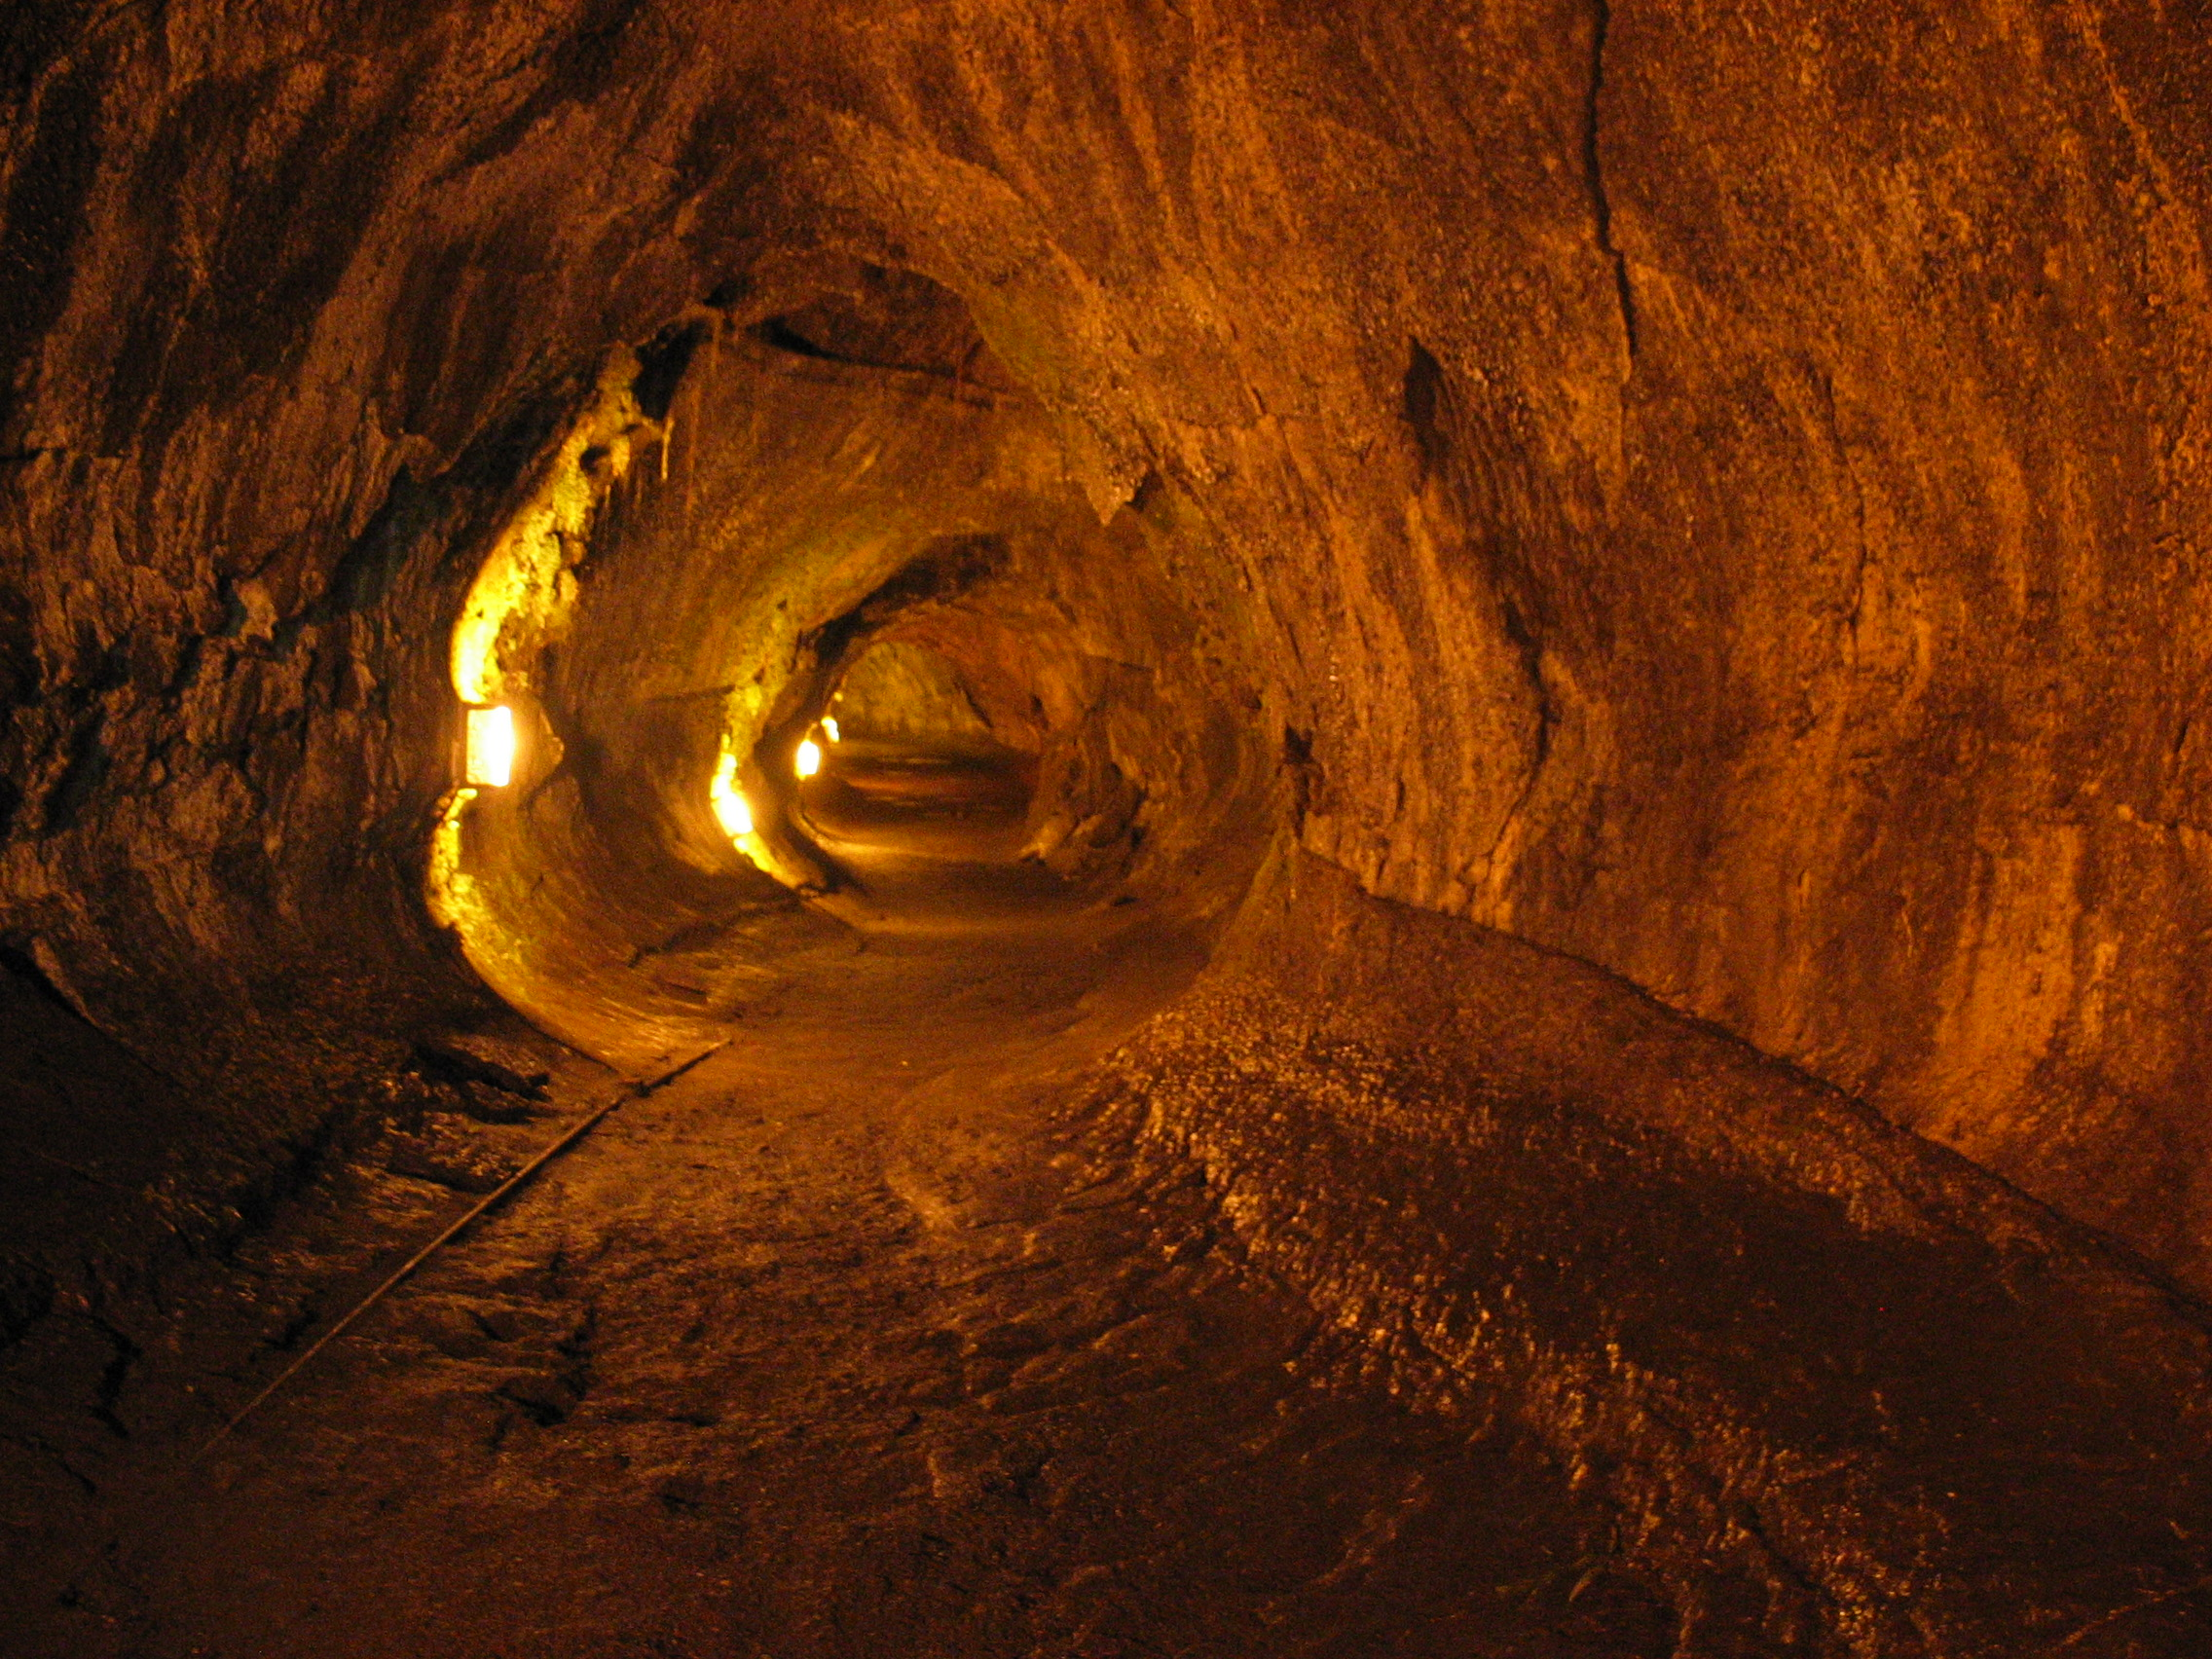
\includegraphics[scale=0.25]{LateX/Images/lavatube.jpg}
        \caption{A lava tube on the isle of Hawaii\cite{lavatube}}
    \end{center}
    \end{minipage}
  \end{figure}
\begin{figure}[!ht]
  \begin{minipage}[c]{0.50\linewidth}
    \begin{center}
      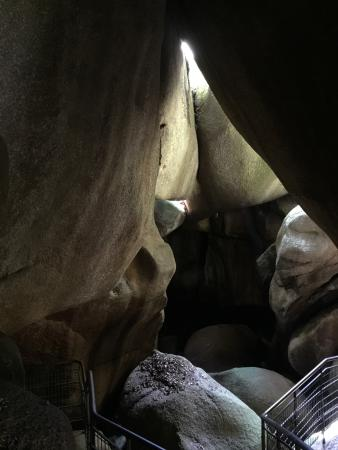
\includegraphics[scale=0.4]{LateX/Images/la-grotte-du-diable.jpg}
      \caption{A blockfield cave in Brittany: ``La Grotte du Diable''\cite{blockfieldcave}}
    \end{center}
\end{minipage} \hfill
\begin{minipage}[c]{0.50\linewidth}
  \item \textbf{Gaps inside blockfield}: Blockfield are old geological formations. Magmatic rocks such as granite cool during their formation. As a consequence, they crack. Then, thanks to the phenomenon of erosion, they are sometimes set on the surface. Moreover, some impure rocks can get into the gaps of the rock. These huge blocks can collapse, particularly in alpine zones, for the impure rocks between the block of magmatic rocks are brittle. This forms a blockfield. Thanks to the collapse and the phenomenon of erosion, some places between the blocks of the blockfield become empty.
  \end{minipage}
\end{figure}

\begin{figure}[!ht]
  \begin{minipage}[c]{0.50\linewidth}
    \item \textbf{Taffoni} (\emph{tafone} in corsicican: hole): These caves are small and look more like empty spaces inside massive blocks of magmatic rocks like granite, or sedimentary rocks, such as sandstone. These kind of caves can only be formed if the climate is dry. Besides the holes are only present on the shadowy part of the rock. Indeed, the difference of humidity and temperature between the shadowy and the sunny parts of the rock, that is already brittle, can disaggregate the rocks. Consequently, the shadowy side of the rock may be dug slowly, as illustrated in Figure 3.
  \end{minipage}\hfill
  \begin{minipage}[c]{0.50\linewidth}
  \begin{center}
    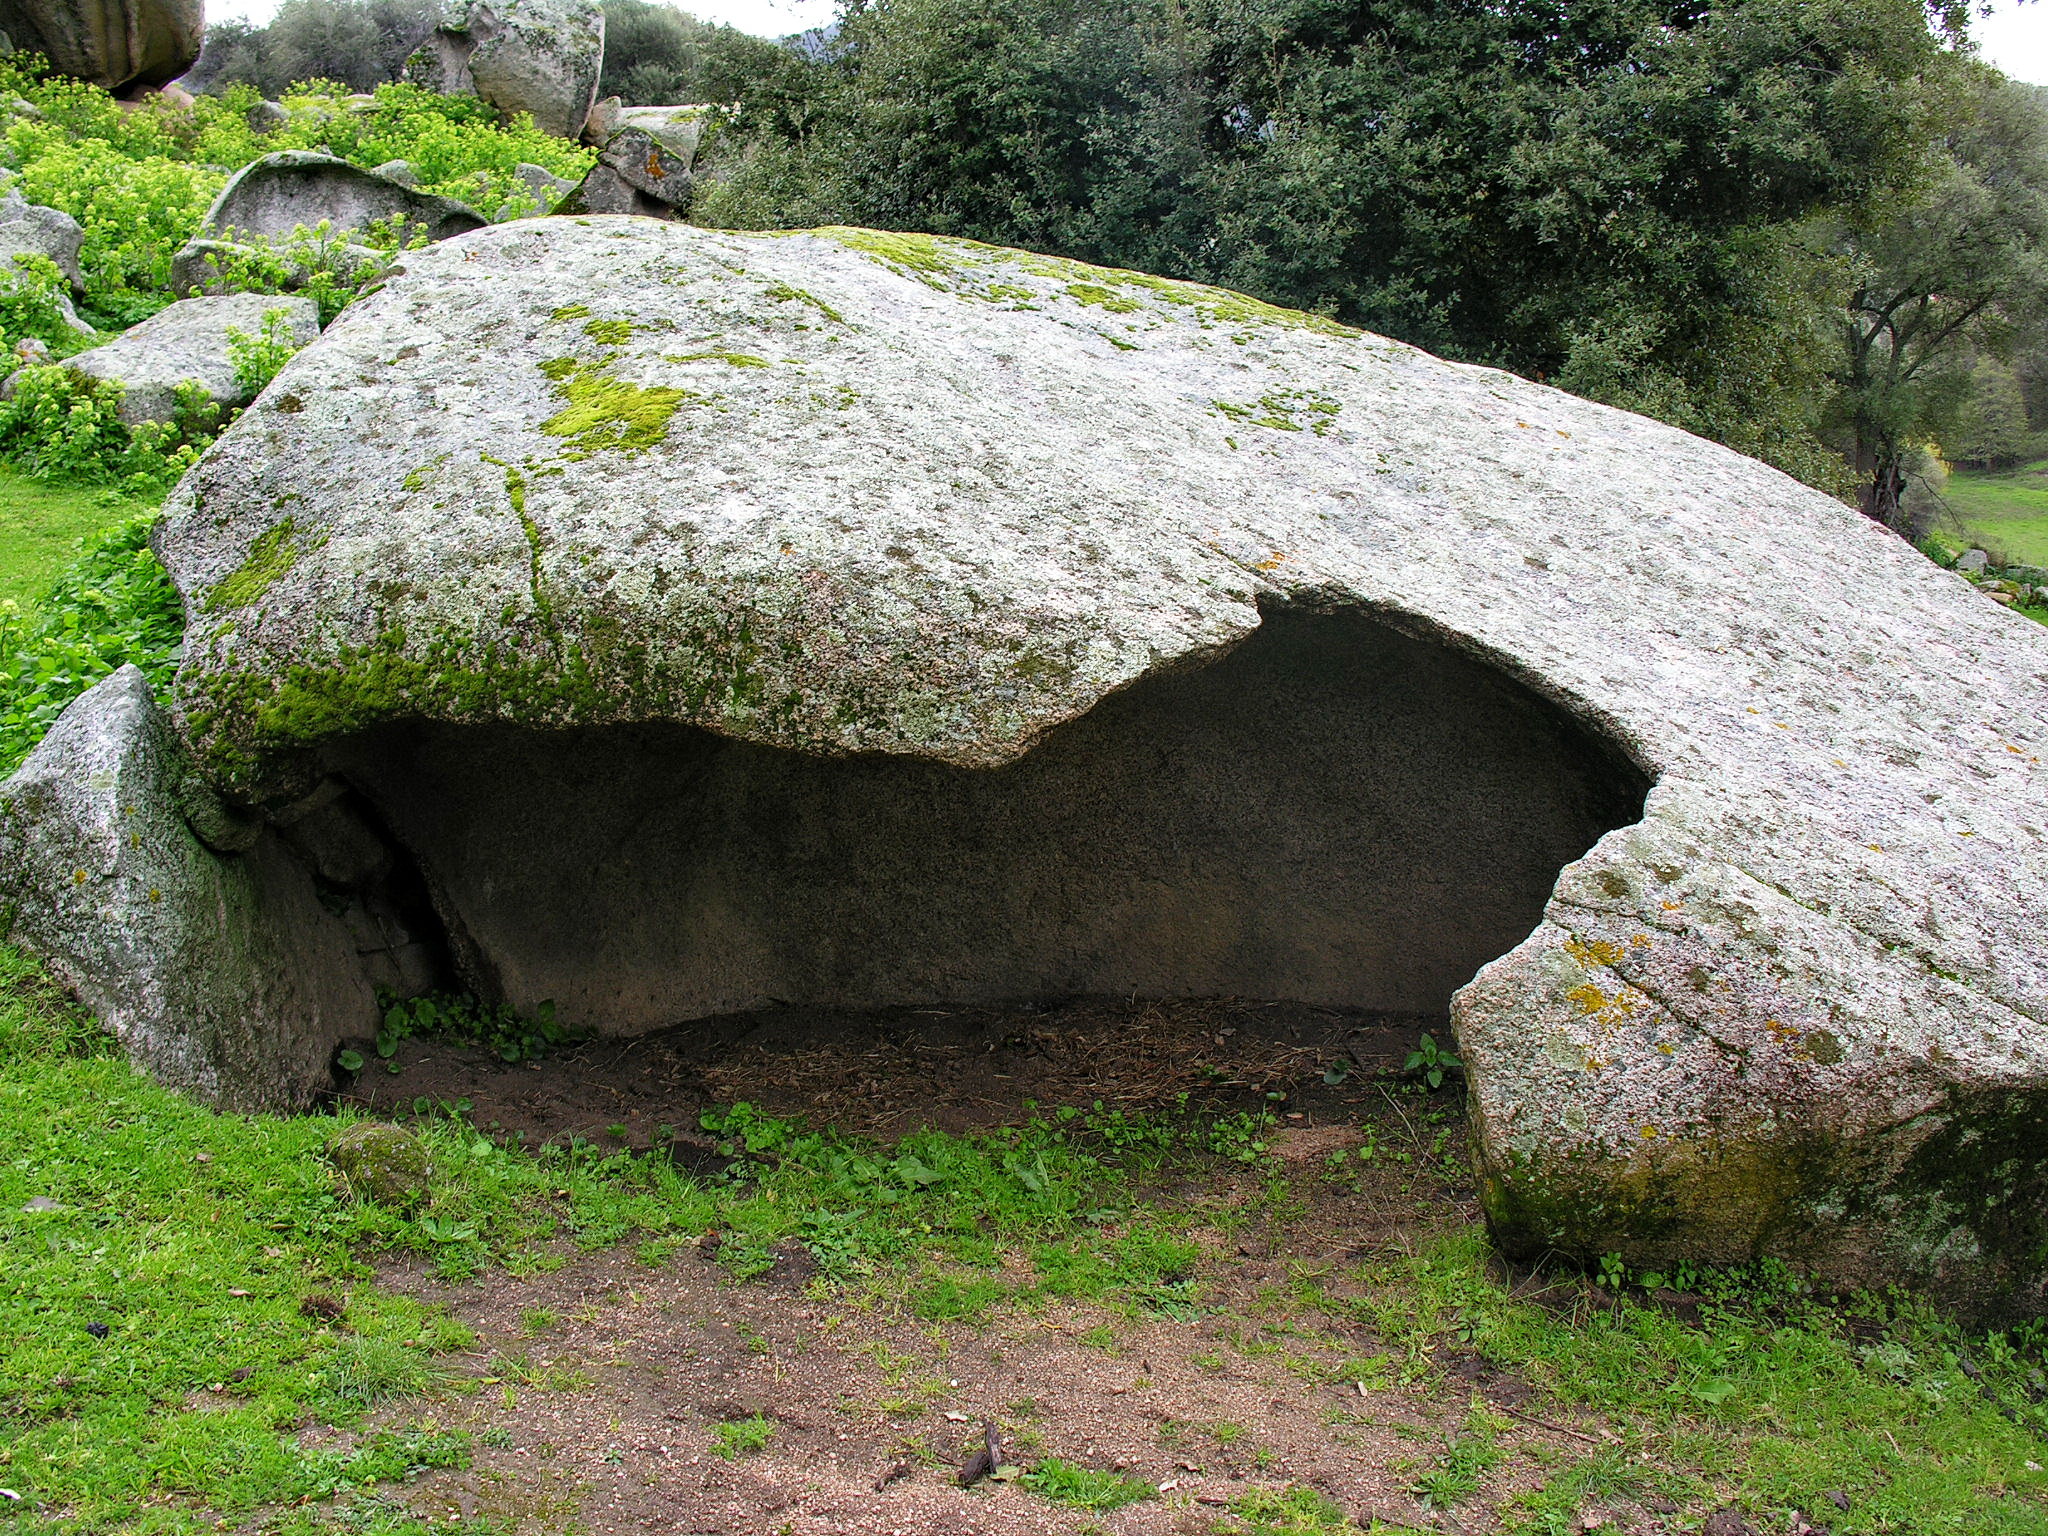
\includegraphics[scale=0.4]{LateX/Images/taffoni.jpg}
    \caption{A taffoni formation in Corsica\cite{taffoni}}
  \end{center}
\end{minipage}
\end{figure}

\begin{figure}[!ht]
  \begin{minipage}[c]{0.50\linewidth}
    \begin{center}
      \includegraphics[scale=0.06]{LateX/Images/subglacialcave.jpg}
      \caption{a huge cave inside the Nigardsbreen glacier, Norway\cite{subglacialcave}}
    \end{center}
  \end{minipage}\hfill
  \begin{minipage}[c]{0.50\linewidth}
      \item \textbf{Subglacial caves}: These caves are formed in volcanic environments and generally in very cold environments, like in Iceland. A hot spring, due to the volcanic activity can dissolve the ice upon it, even if this ice is very thick. This phenomenon is very quick, contrary to the other types of cave’s formation. However, the lifetime of these caves is very short too. Indeed, ice is known as very fragile, and can collapse easly.
  \end{minipage}
\end{figure}

\end{itemize}
\break
However, the vast majority of caves were formed in a rather limited types of rocks called karstic rocks. They cover approximately 12 percent of the ice-free landmass, with China having the largest surfaces.\\
In the world we have found a lot of caves (about 10000) .\\

\chapter{Karst Rocks}
~\par
All rocks are soluble, that is to say they can be dissolved, thus the chemical species that compose these rocks are able to be separated by a liquid solution of a specific species. But some rocks are much more soluble into natural acids that are present at the surface of the Earth. Acids do have a pH\footnote{pH stands for Potential Hydrogen} between 0 and 7. It means that inside those liquids, $H^{+}$ ions are more present than $HO^{-}$ ions. Carbonic acid is the most abundant of these acids because rainwater in combination with carbon dioxide (mainly from the soil including its bacteria) becomes a mild carbonic acid (soda). Obviously, salts of the carbonic acid are dissolved according to the following generic reaction :\\

\begin{chemmath}
  CaCO_3(s) + H_2CO_3 (l) \leftrightharpoons Ca^{2+}(aq) + 2HCO_3^{-}(aq)
\end{chemmath}
The chemical species formed by the dissolution are no more molecules or atoms, but ions, since they get or lose some electrons. Here, there are two ions, a cation ($Ca^{2+}$), that lost two electrons (two negative charges), and thus has a positive charge, and two anions ($HCO_{3}^{-}$), that got one electron, thus have now a negative charge.
This special phenomenon of dissolution is called the \textbf{solubilization}.\\
\par
Sedimentary carbonates are in fact a continuous range of mixtures of various minerals with impurities. Indeed, they were formed in millions of years, on the ground of the oceans, the lakes, the rivers and the seas. The accumulation of layers of different sands leads to the solidification of these sands. The solidification of these rocks is due to the fact that over time, the layers go down into the ground and are covered by more recent layers. Consequently, they become solid because of the high pressure of the other layers.\\
\begin{figure}[!ht]
  \centering
  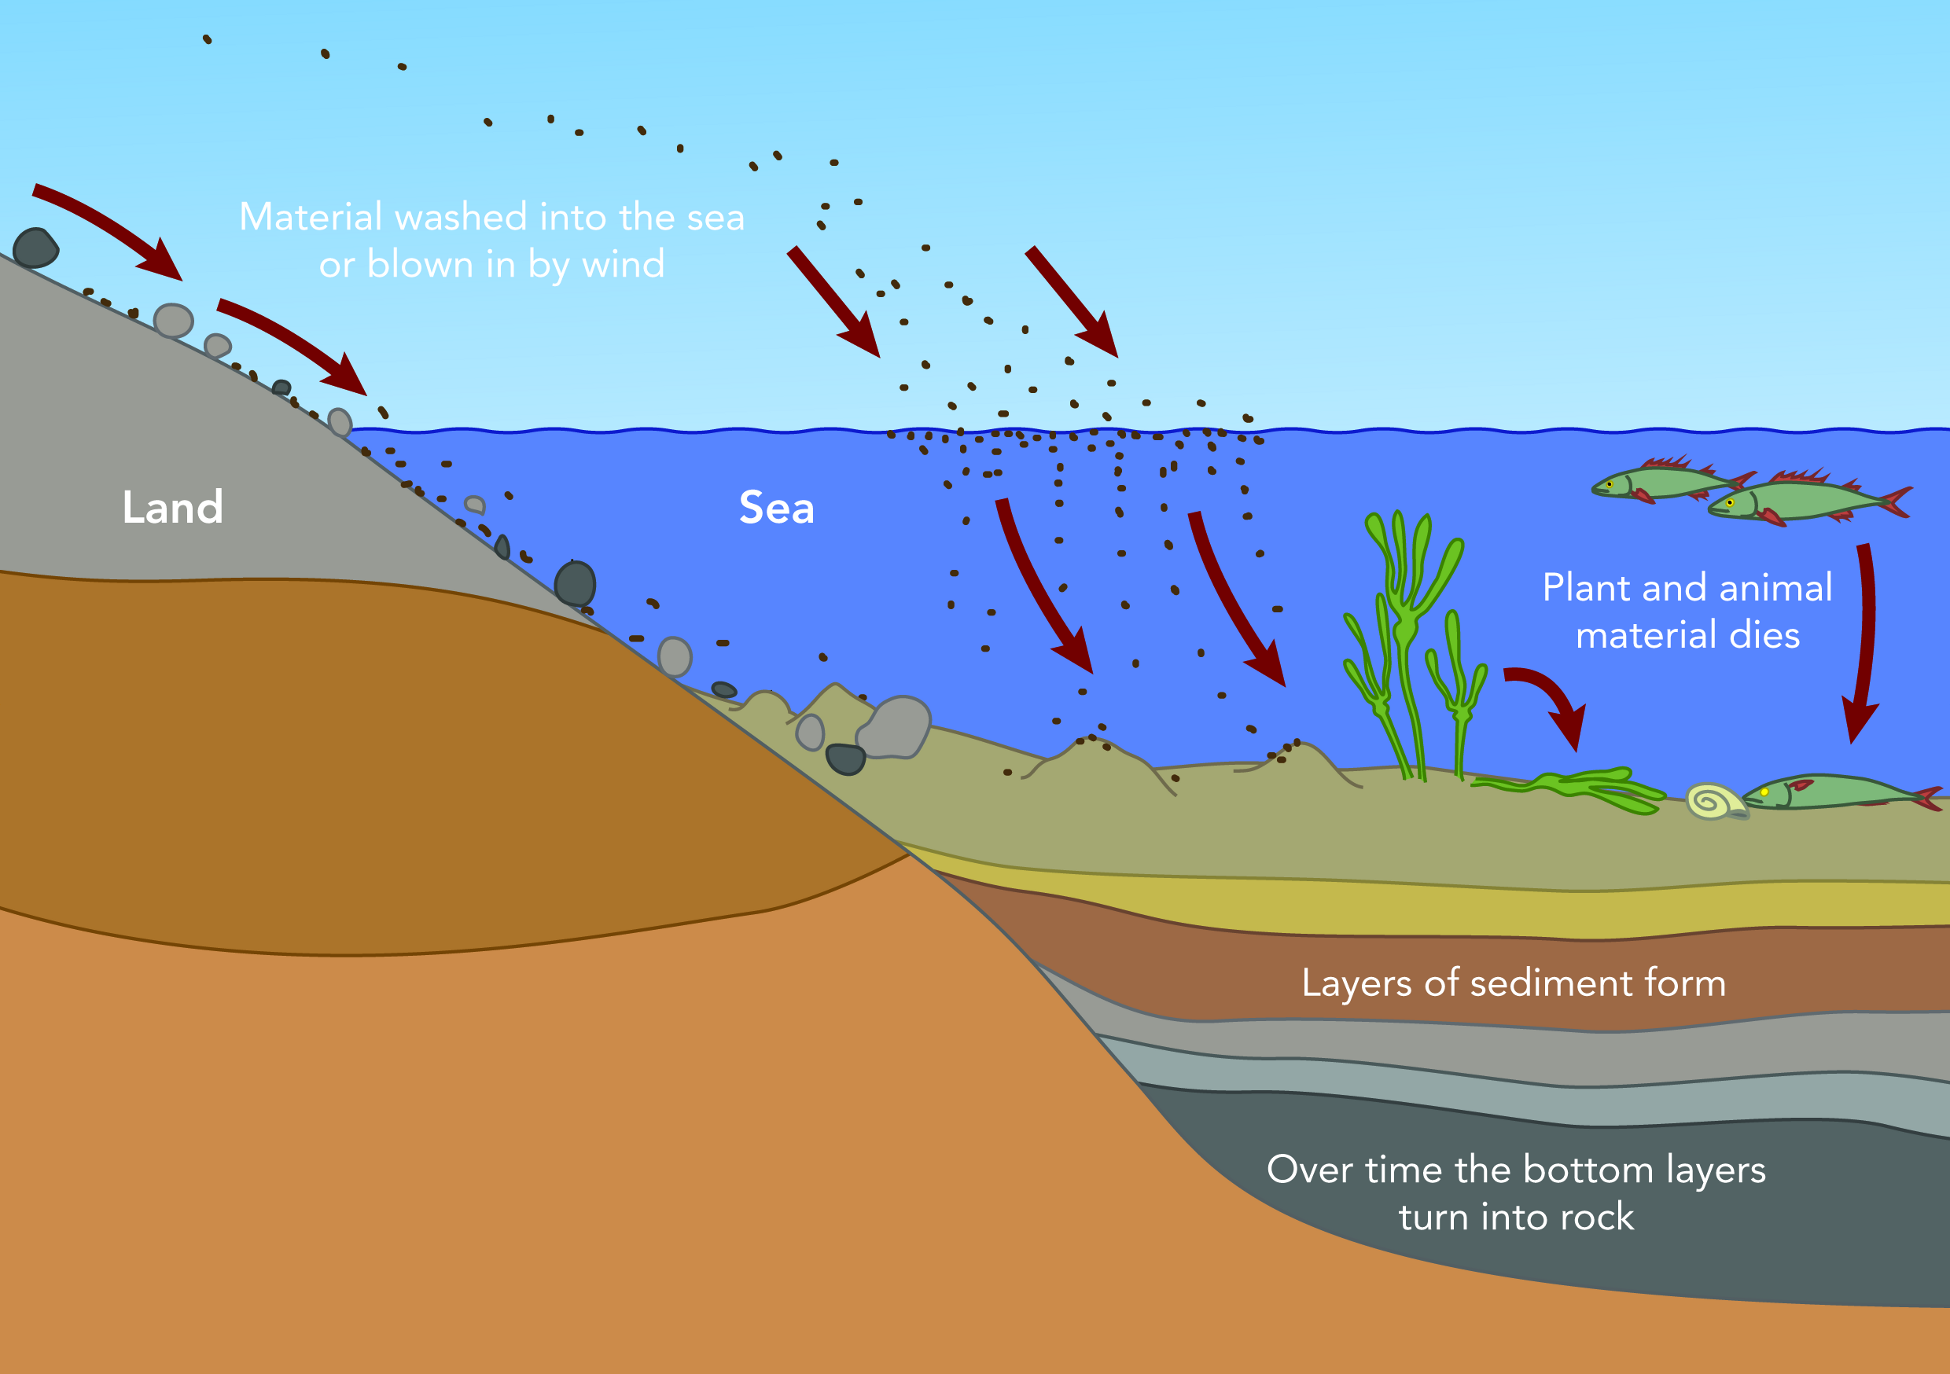
\includegraphics[scale=1]{LateX/Images/sedimentaryrock.png}
  \caption{Scheme of the formation of sedimentary rocks, like limestone\cite{sedimentaryrocks}}
\end{figure}
Limestone is built mostly of calcium carbonate and is the easiest to dissolve. The mineral dolomite is a double carbonate of calcium and magnesium  and it is believed to form the calcite lattice by the addition of magnesium atoms. How that addition occurs is very poorly understood and is still a matter of debate. Surprisingly, when it occurs, although new atoms are introduced into the lattice, the result is shrinkage, which will fracture the dolomitized rock, increasing its porosity ! The dolomite rock is never made of pure dolomite. The dolomite mineral is slightly less soluble than calcite. There are significantly more referenced limestone than dolomites caves (for the same volume of rock).  The reason for such a difference lies in the dolomite's tendency to crumble into fine dust (sometimes termed « dolomite flour ») because of the jagged contour of the dolomite crystals (which first dissolve at the pointed tips, thus loosening the support between adjacent crystals). The calcite crystals in the limestone, on the contrary, have linear contours and they dissolve in depth without crumbling at a microscopic scale.\\

All karst features that occur in carbonate rocks mainly by dissolution are sometimes referred as orthokarst (true karst). \\

Other types of sedimentary rocks also host many caves, some of them very large. Rock gypsum (calcium sulphate with two water molecules) is such a rock and also rock salt, both referred to as evaporite rocks (because they are believed to have been laid down by the evaporation of salty  seawater). Evaporite rocks are however usually very pure, which suggests they were not deposited by evaporation. In fact, if they would have been exposed to the sun's heat, they should have been mixed with many other sediments. The best assumption could be a rapid deposition in complex chemical underwater conditions generated by a submarine volcanic activity.

\chapter{Cave formation}
~\par
Caves are formed by the dissolution of limestone. Rainwater picks up carbon dioxide from the air and percolates through the soil. The addition of water and carbonic acid turns then into a weak acid. This acid slowly dissolves out the limestone along the joints, bedding planes and fractures, some of which become enlarged enough to form caves. The largest caves form where water flows onto the limestone from the adjacent impermeable Portishead Formation (Old Red Sandstone) and Avon Group mudstones. The water sinks underground into holes known locally as ``swallets'' or ``slockers''. The streams reappear at the base of the limestone outcrop at large springs, for example at Cheddar and Wookey Hole. Over time, the water finds new lower routes leaving some caves high and dry. Some cave entrances have been dug out by spelunkers.
\begin{figure}[!ht]
  \centering
  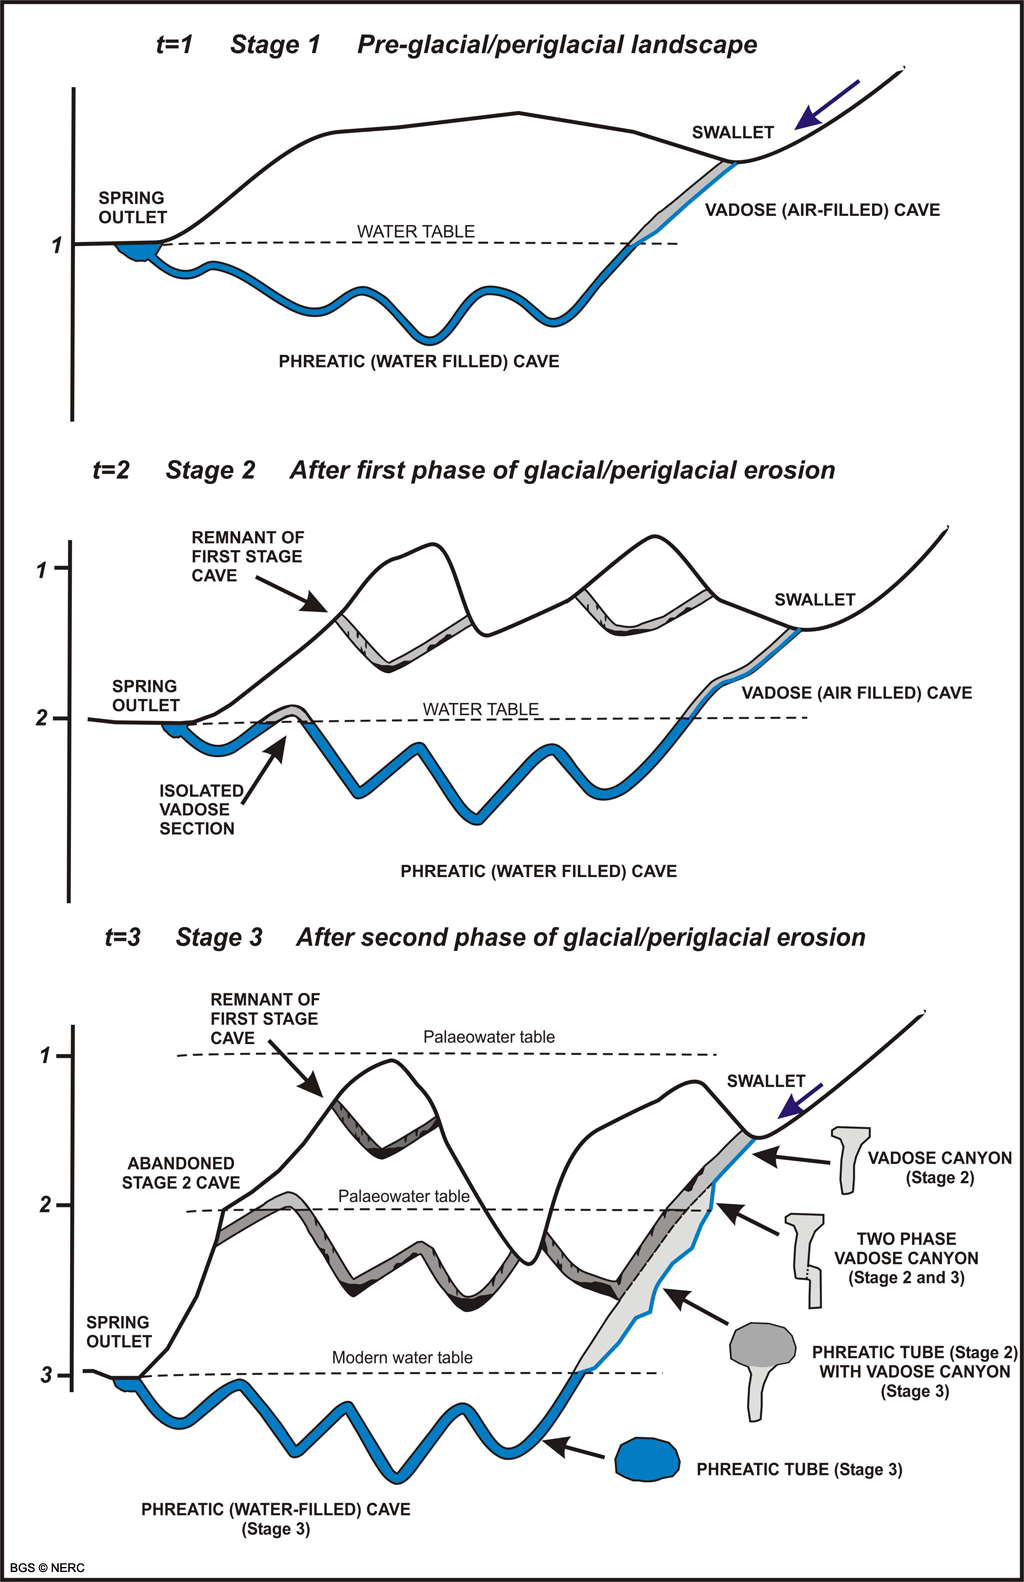
\includegraphics[scale=0.4]{LateX/Images/schemekarstformation.jpg}
  \caption{Scheme of the formation of a karst cave\cite{caveformationscheme}}
\end{figure}
\clearpage
\section{Unusual caves}
~\par
There are many different types of caves. In order to illustrate this affirmation, this chapter will introduce some unusual caves.\\
\begin{itemize}
  \item \textsc{Cave of Crystals} (Mexico): this cave is totally covered with crystals (as indicated by it name). This cave is one of most recently discovered caves of the world, the Crystal Caves were discovered in 2000 after drilling in an aquifer, and pumping out tens of thousands of gallons of water. The crystal formations are mind bogglingly large, some measuring over 30 feet in length and 4 feet in diameter.
  \begin{figure}[!ht]
    \centering
    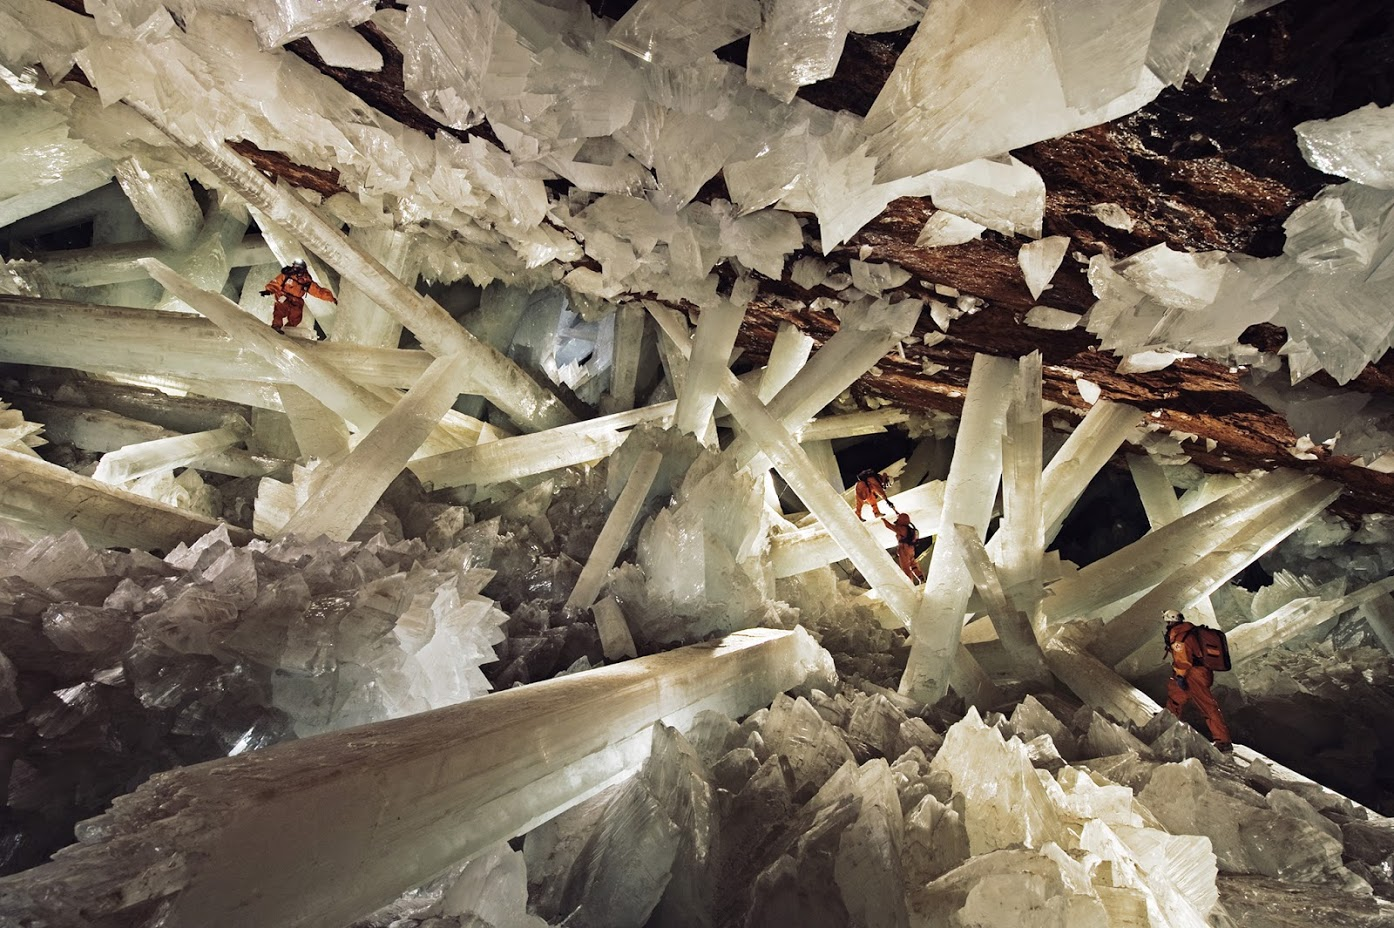
\includegraphics[scale=0.15]{LateX/Images/crystalcave.jpg}
    \caption{Photography of tha Cave of Crystals\cite{naicacave}}
  \end{figure}
  \item The second cave is \textsc{Mammoth Cave} (USA). It's one of the oldest and most well known caves in the United States, located in central Kentucky. Mammoth Cave boasts to be the longest in the world with over 365 miles of subterranean passageways. The cave was “discovered” by American settlers in the late 18th century, but was well known to local Native Americans long before. The cave became a National Park in the summer of 1941. There are spectacular sights such as a giant sinkhole called “Cedar Sink” or “Frozen Niagara”.
  \begin{figure}[!ht]
    \centering
    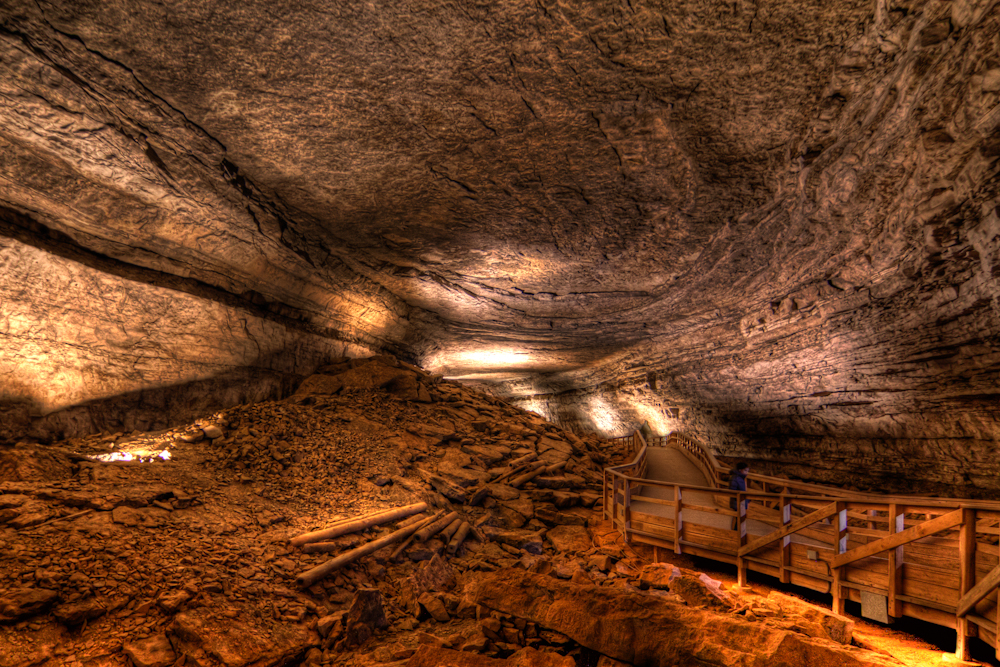
\includegraphics[scale=0.7]{LateX/Images/mammothcave.jpg}
    \caption{Photography of the Mammoth Cave\cite{mammothcave}}
  \end{figure}
    \clearpage
  \item The third and the last is \textsc{Mulu Caves} (Borneo). The caves beneath Mulu National Park, so far, cover over 125 miles. Though some say that it is possible that there’s three times that distance waiting to be discovered. According to the Sarawak Forestry Department, Mulu Caves has the largest passage, the largest chamber, and the longest cave in Southeast Asia. This cave is very touristic and tours are organized for  beginner to experienced spelunkers.
  \begin{figure}[!ht]
    \centering
    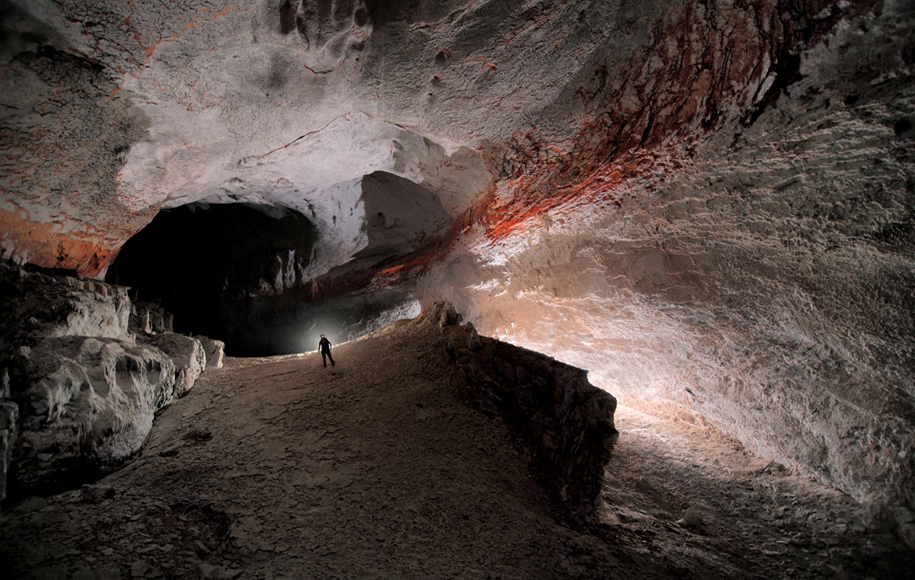
\includegraphics[scale=0.3]{LateX/Images/mulucave.jpg}
    \caption{Photography of the Mulu Cave\cite{mulucave}}
  \end{figure}
\end{itemize}


\chapter{Special Features of Karst Caves : Stalactites/Stalagmites}
~\par
 The words stalactite and stalagmite have been introduced by the Greeks with the words ``stalassein'', which means ``to drip''. It describes how both are formed in nature. Although they look lifelike and a little creepy, stalactites and stalagmites grow slowly due to water running over and through inorganic material.\\

Limestone caves, where most stalactites and stalagmites can be found, are mainly composed of calcite, a common mineral found in sedimentary rocks. Calcite molecules are based on calcium and carbonate ions, and are defined as $CaCO_{3}$, or calcium carbonate. When rainwater falls over a cave and trickles through rocks, it takes along carbon dioxide and minerals from limestone. If we add water, carbon dioxide and calcium carbonate together, we get this equation:\\
\begin{chemmath}
  H_2O(l) + CO_2(g) + CaCO_3(s) \longrightarrow Ca(HCO_3)_2(aq)
\end{chemmath}
But then, limestone, under aqueous form, turns into solid limestone, because of the lack of $CO_{2}$ in the caves, due to the dissolution of the limestone. The formation of stalactite can also be explained by the alternation of two phases, using the same reaction in both senses.\\
Stalactites start as tiny tubes that over time increase in diameter until they become more or less conical in shape. They mostly preserve their central tube, being constantly supplied with drip water. In a few cases, the original tube retains its diameter and a soda straw (tubular stalactite) will start growing. This tiny, translucent calcite tube can exceptionally reach several feet in length ! In most cases, thought, such tubes break under their own weight. The process of formation of stalactites and stalagmites is depicted in Figure 3.4.

Stalagmites are deposited one layer on top of the other, usually thicker at the base and narrowing toward the tip. Their shape and size varies enormously, some reaching tens of feet in height. Of course, stalagmites don't just emerge from the ground. The water dripping from the end of a stalactite falls to the floor of a cave and deposits more calcite into a mound. Soon enough, a stalagmite will form in a cone-like shape.\\
Stalagmites do not possess a hole inside, because they are just formed by the accumulation of water, saturated with limestone, that turns into solid limestone because of the solubilization phenomenon.\\

This is why we usually find stalactites and stalagmites in pairs, and sometimes they'll even grow together to form one big column(\ref{column}). There are many limestone caves around the world famous for their displays of dripstone, including Carlsbad Caverns in New Mexico, Timpanogos Caves in Utah, Mammoth Cave in Kentucky and Jenolan Caves and Buchan Caves in Australia.\\
  \begin{figure}[!ht]
      \begin{minipage}[c]{0.50\linewidth}
        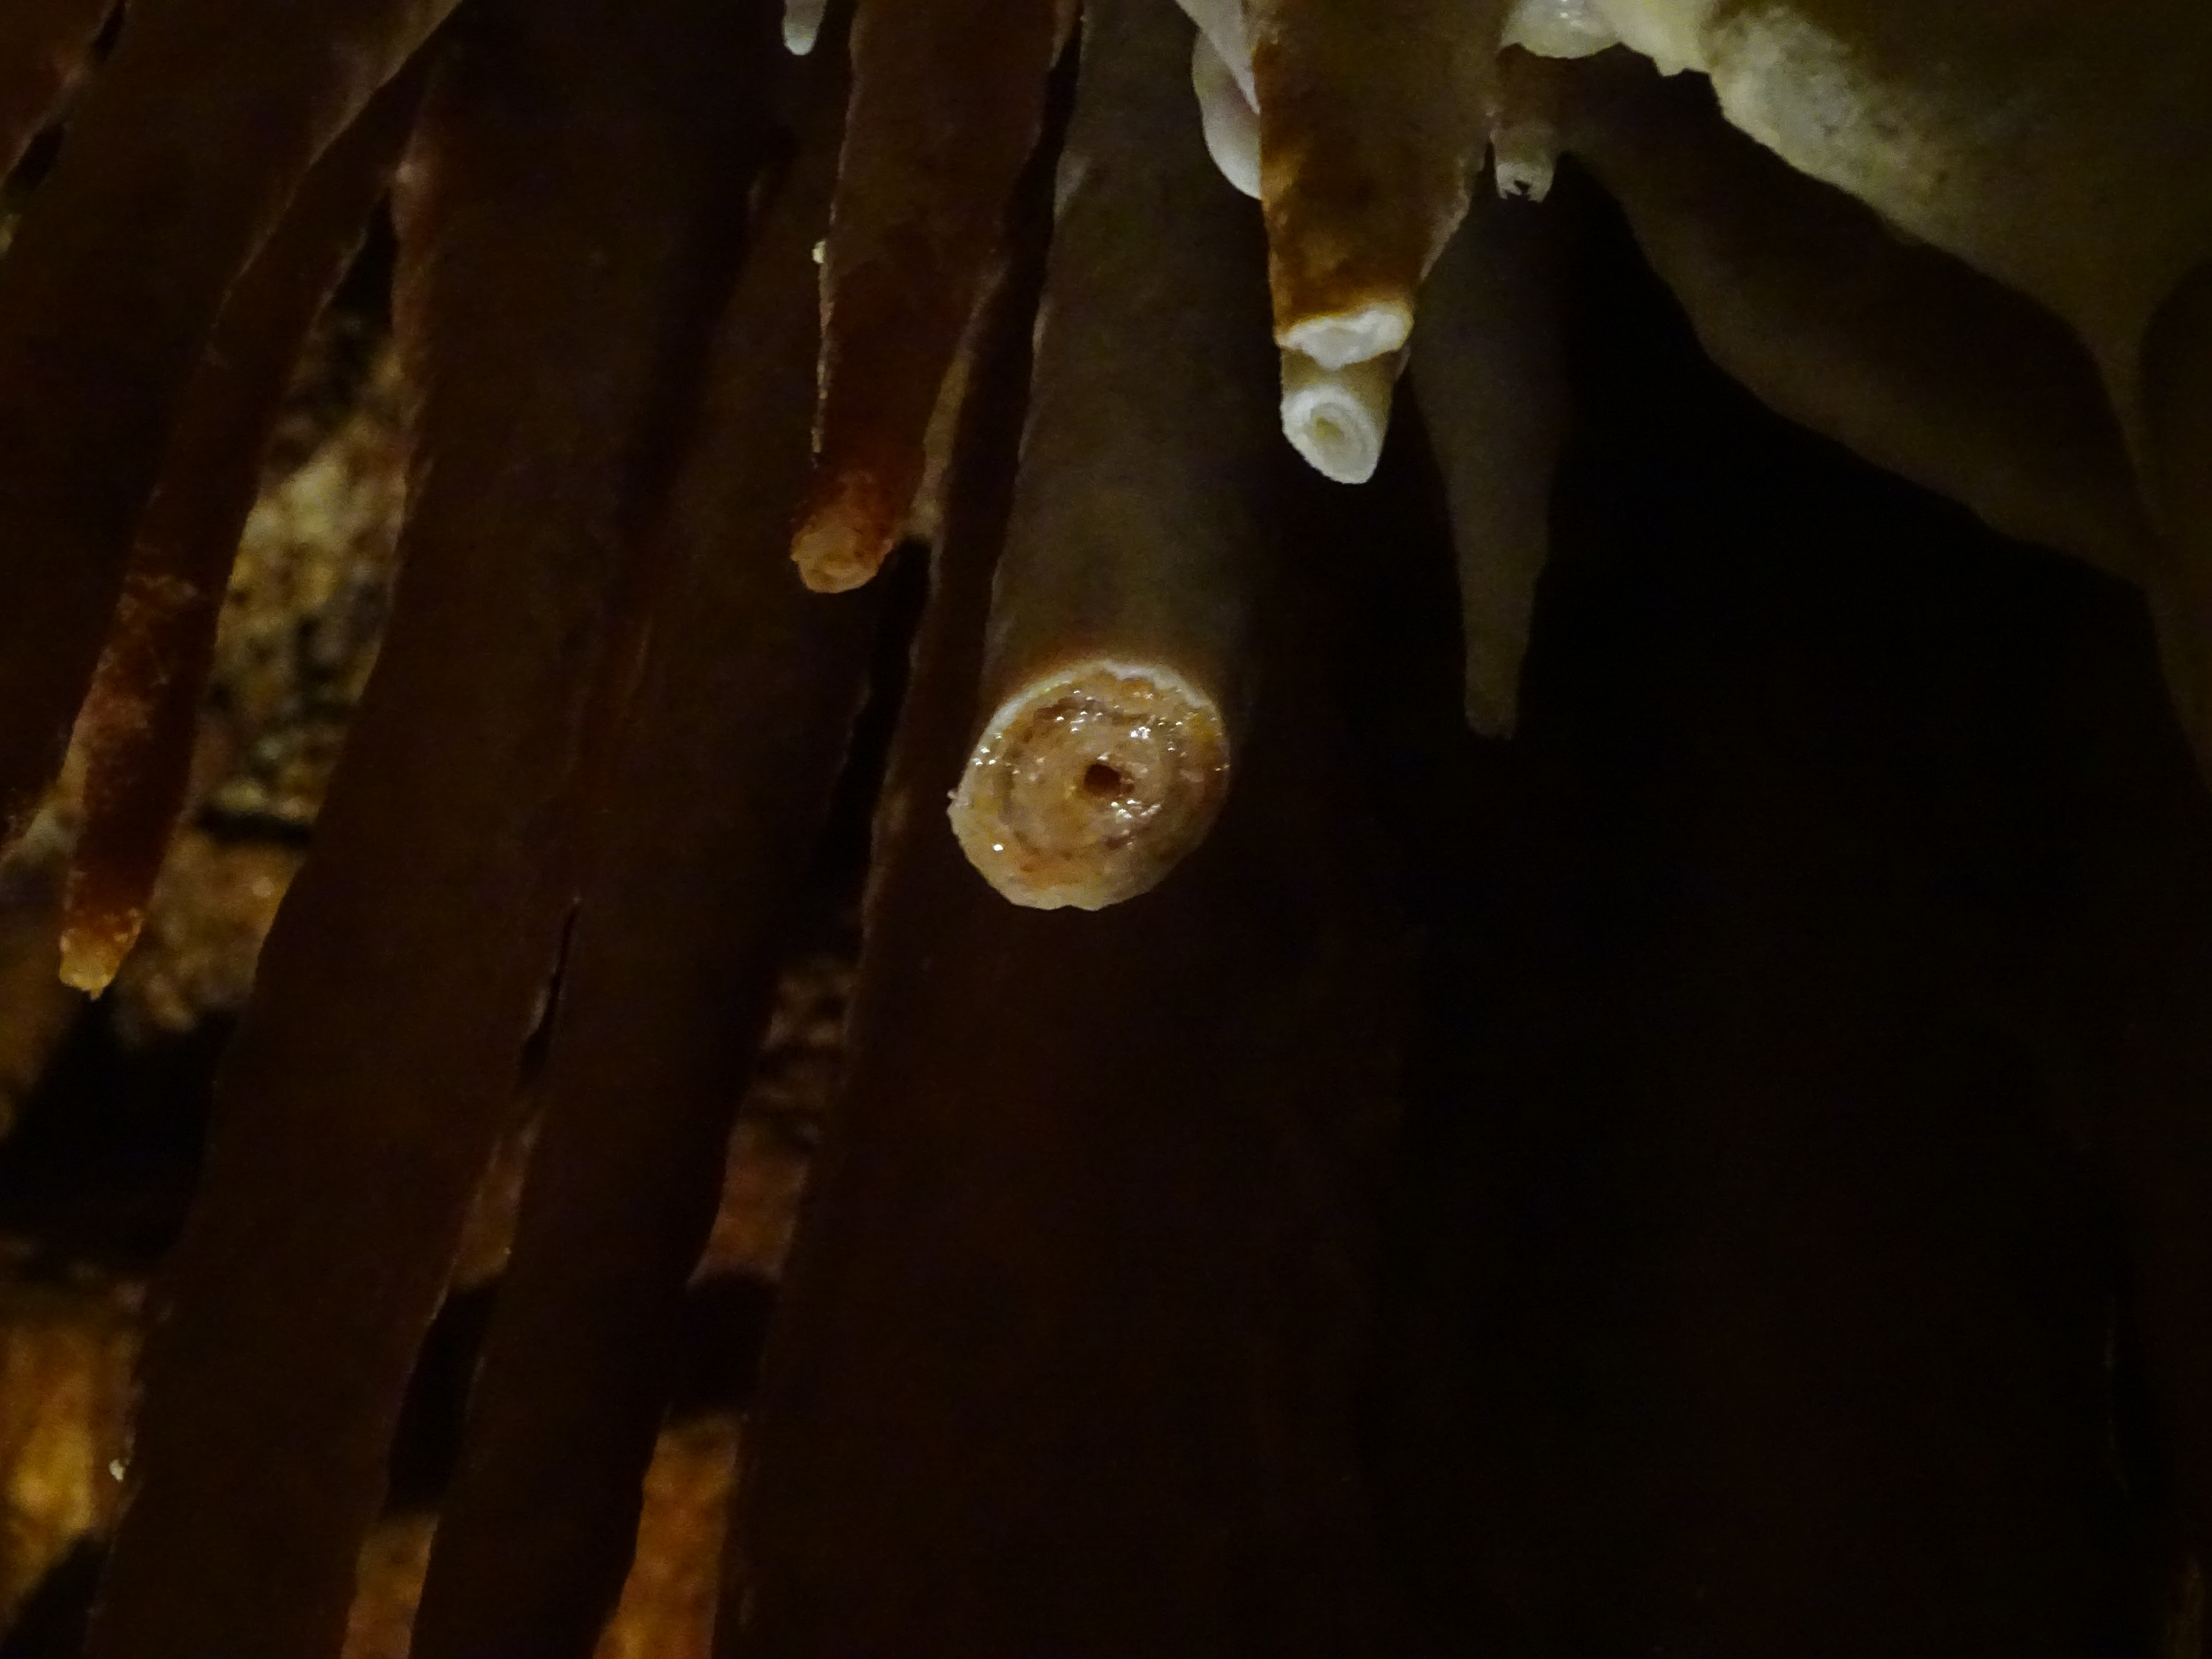
\includegraphics[scale=0.22]{LateX/Images/stalagmitesolubilization.jpg}
        \caption{Inside of a stalactite in the cave of Fontrabiouse}
      \end{minipage}\hfill%
    \begin{minipage}[c]{0.50\linewidth}
      \includegraphics[scale=0.22]{LateX/Images/macaroni.jpg}
      \caption{Soda straws on the ceiling of the cave of Fontrabiouse}
    \end{minipage}
\end{figure}
\begin{figure}[!ht]
  \centering
  \rotatebox{90}{\includegraphics[scale=0.2]{LateX/Images/column.jpg}}
  \caption{A huge column in the cave of Fontrabiouse\label{column}}
\end{figure}

\begin{figure}[!ht]
  \centering
  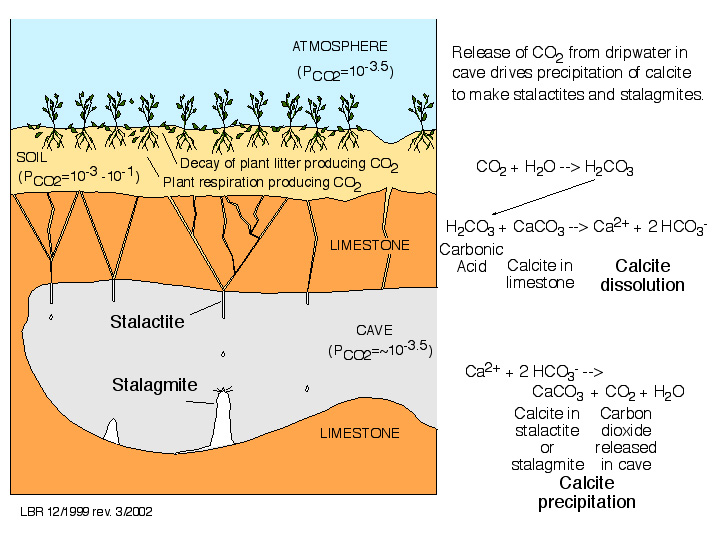
\includegraphics[scale=0.7]{LateX/Images/stalactitescheme.jpg}
  \caption{Scheme of the formation of stalactites and stalagmites in Karst cave\cite{stalactiteformationscheme}}
\end{figure}
\clearpage
  \paragraph{Experimental protocol}
  \subparagraph{Introduction}
  We will form a salt stalagtite. We will see later how the phenomenon of formation of a salt stalactite can be linked to the formation of a calcite stalagtite. We will try to reproduce the slow stalactite creation process and study the influence of the environment differences on this process.

\textbf{equipment}
\begin{itemize}
  \item 4 beakers
  \item 1 spoon
  \item 2 ropes
  \item 1 spoon
  \item warm water
  \item food coloring
  \item sodium bicarbonate ($NaHCO_{3}$)
  \item 2 plates
\end{itemize}

\textbf{Protocol} \\
Before the experiment
    \begin{enumerate}
      \item Pour 200mL of warm water in each beaker.
      \item In 2 beakers, put 5 spoonful of sodium bicarbonate (40g). In the two other, put only 2 spoonful of it (20g).
      \item Agitate to dilute the sodium bicarbonate in each beaker.
      \item Fold the ropes to form a M shape rope.
      \item In front of both montages, put a camera, perpendicular to the floor, parallel to the montages. Add a ruler, in order to be able to mesure the size of the stalactite by only looking at the pictures.
      \item Programm the camera to make it take two frame a day.
      \item Wait about one or two weeks (depending of the growth of the stalactite.
    \end{enumerate}

    \begin{figure}[!ht]
      \centering
      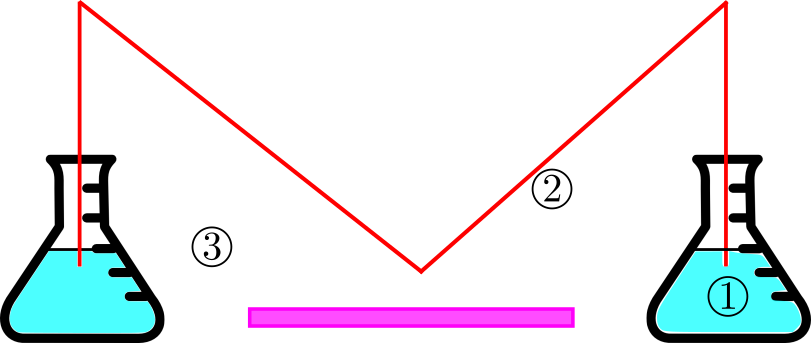
\includegraphics[scale=0.3]{LateX/Images/schemeexperiment.png}
      \caption{ \textsc{Scheme of the experiment}\\
                1. Beaker containing water and sodium bicarbonate ($NaHCO_3$), at different concentrations\\
                2. Ropes (wool)\\
                3. Plate\\}
    \end{figure}
\break
\textbf{After the experiment}
\begin{enumerate}
  \item After one or two weeks, compare the size of both stalactites.
  \item Draw the graph of the size of the stalactite according to time, by using the frames of the camera for both stalactite.
  \item Make observations and try to conclude.
  \item Look more accurately at the stalactite, try to identify crystals (take accurate photos).
  \item Break the stalactite in order to make observations of the inside (take accurate photos).
\end{enumerate}



\paragraph{Observations}
~\newline
\emph{Note: The experiment was realized inside a kitchen (Temperature $\simeq$ 20°C; Pressure $\simeq$ 1013 hPa)}

\begin{figure}[!ht]
  \begin{minipage}[c]{0.50\linewidth}
    We can observe at the beginning of the experiment that, the 40g sodium bicarbonate are not totally dissolve compared  with the glasses which contained 20g of.
  \end{minipage}\hfill
  \begin{minipage}[c]{0.50\linewidth}
  \begin{center}
    \includegraphics[scale=0.2]{LateX/Images/startexperiment.jpg}
    \caption{beginning of the experiment: $h=0 hours$}
  \end{center}
\end{minipage}
\end{figure}

\begin{figure}[!ht]
  \begin{minipage}[c]{0.50\linewidth}
    \begin{center}
      \includegraphics[scale=0.2]{LateX/Images/11hexperiment.jpg}
      \caption{State of the experiment after 11h: $h=11 hours$}
    \end{center}
  \end{minipage}\hfill
  \begin{minipage}[c]{0.50\linewidth}
    We can notice that some crystals  appeared on the rope between the glasses with 20g of sodium bicarbonate.
  \end{minipage}
\end{figure}

\begin{figure}[!ht]
  \begin{minipage}[c]{0.50\linewidth}
    We can see that some crystals  appeared on the rope between the glasses with 40g of sodium bicarbonate
  \end{minipage}\hfill
  \begin{minipage}[c]{0.50\linewidth}
  \begin{center}
    \includegraphics[scale=0.2]{LateX/Images/1dayexperiment.jpg}
    \caption{State of the experiment after 1 day: $h=24 hours$}
  \end{center}
\end{minipage}
\end{figure}

\begin{figure}[!ht]
  \begin{minipage}[c]{0.50\linewidth}
    \begin{center}
      \includegraphics[scale=0.2]{LateX/Images/8dayexperiment.jpg}
      \caption{State of the experiment after 8 days: $h=192 hours$}
    \end{center}

  \end{minipage}\hfill
  \begin{minipage}[c]{0.50\linewidth}
    We can observe that after 8 days the crystals stopped their growth. The difference between the 2 concentrations can be explained by the difference of dissolution at the beginning of the experiment.
  \end{minipage}
\end{figure}

% Ici insérer les graphiques + conclusions sur l'expérience.
% Explication graphiques
Actually, the reaction that occurs in the formation of this stalactite is not really the same as the one which occurs in caves. Indeed, here water and solid powder of sodium bicarbonate ($NaHCO_3$) react together. Besides, the reaction is far more simple than the solubilization, occuring inside caves. The sodium bicarbonate is only dissoluted. We also have the following reaction:
\begin{chemmath}
  NaHCO_{3}(s) \longrightarrow Na^{+}(aq) + HCO_{3}^{-}(aq)
\end{chemmath}
The problem is, that the water is saturated with sodium bicarbonate. Thanks to the phenomenon of capillary, water rises up to the rope, and then slides down and falls between the two glasses.
Even if the phenomenon does not look like the one that create stalactites, the result is nearly the same. The sodium bicarbonate settles following the same way as the limestone during the formation of the stalactite. This experiment can also form stalagmite, on the plate, opposite to the stalactite. Furthermore, this experiment needs ``only'' one week to form a little stalactite, whereas it takes centuries inside the caves.
\newpage
\begin{figure}[!ht]
  \centering
  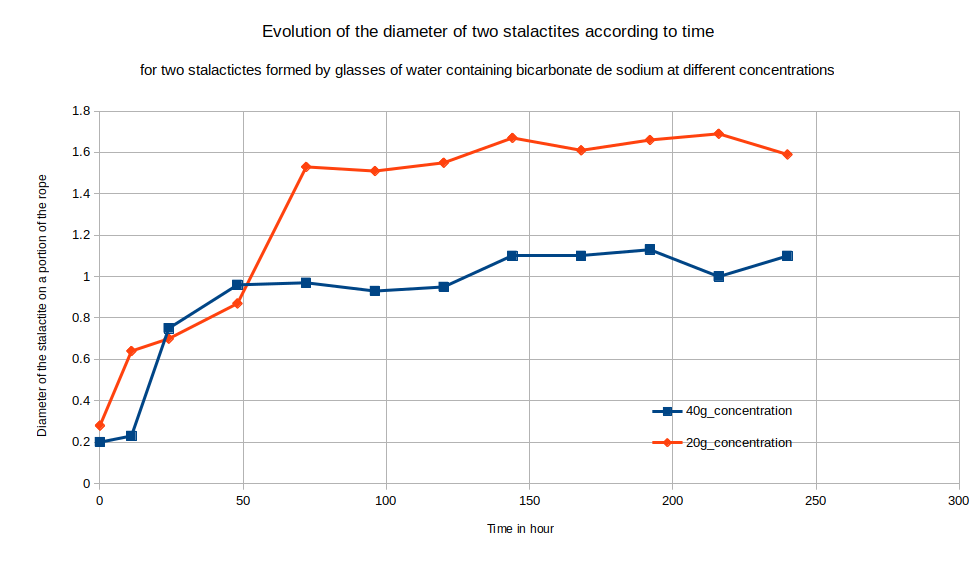
\includegraphics[scale=0.7]{LateX/Images/graphexperiment.png}
  \caption{Graph obtained by measuring the diameter of two stalactites on a slice of the rope}
\end{figure}

On the graph, we can see that first, the 40g-concentrated glasses of water produce faster than the 20g-concentrated ones a stalactite. But after 50 hours, the diameter of the stalactite obtained with the 20g-concentrated glasses of water becomes bigger than the other stalactite. Moreover, at 72 hours, the size of this same stalactite tends to level off around 1.6 - 1.7 centimeter. This stabilisization is due to the lack of saturated water, and the fact, that because solid sodium bicarbonate is already present on the rope, the capillary action becomes slower. In caves, the process of formation of the stalactites is also really long, due also to the water flux that slows with time.\\
\indent However, the size of the stalactite should not reduce during the experiment. The fluctuations are also due to the experiment conditions. Indeed, we fixed one camera in front of the experiment, that has taken photos since the beginning of the experiment. To make the stalactites measurable, we also took all our photos in the same way, with the same shot. Unfortunately, it happended that the stalactites measured turned around the rope, falling because of their weight and the action of the gravity. The days the stalactites rotated, we also measured a smaller diameter with the photo. We decided not to change our figures to realize our graph, for we did want not to invent figures and to adopt a scientific approach, by using our data, even if we knew that they were somewhat wrong.
In caves, a stalactite can all the same loose lenght and weight, because of shocks, for instance when people hit them, or simplier due to earthquake. Furthermore, a stalactite can deteriorate if the rate of $CO_{2}$ increases, because of the phenomenon of solubilization.\\
\par
The other stalactite becomes smaller at the end of the experiment, for the supersaturated water deposed faster solid sodium bicarbonate on the edges of the rope, in contact with the glass. Therefore, there is less solid sodium bicarbonate on the rest of the rope, thus less and smalles stalactites.\\
\par
\textbf{Note:} We produced the experiment twice, but the second time we were not able to take regular photos. This experiment was the same except the plate, replaced by a cup. After two weeks, a stalagmite formed inside the cup, opposite to a stalactite, exactly like in caves.\\
\newpage
% Insérer photo de l'expérience bis aves le stalagmite en évidence.
\begin{figure}[!ht]
  \centering
  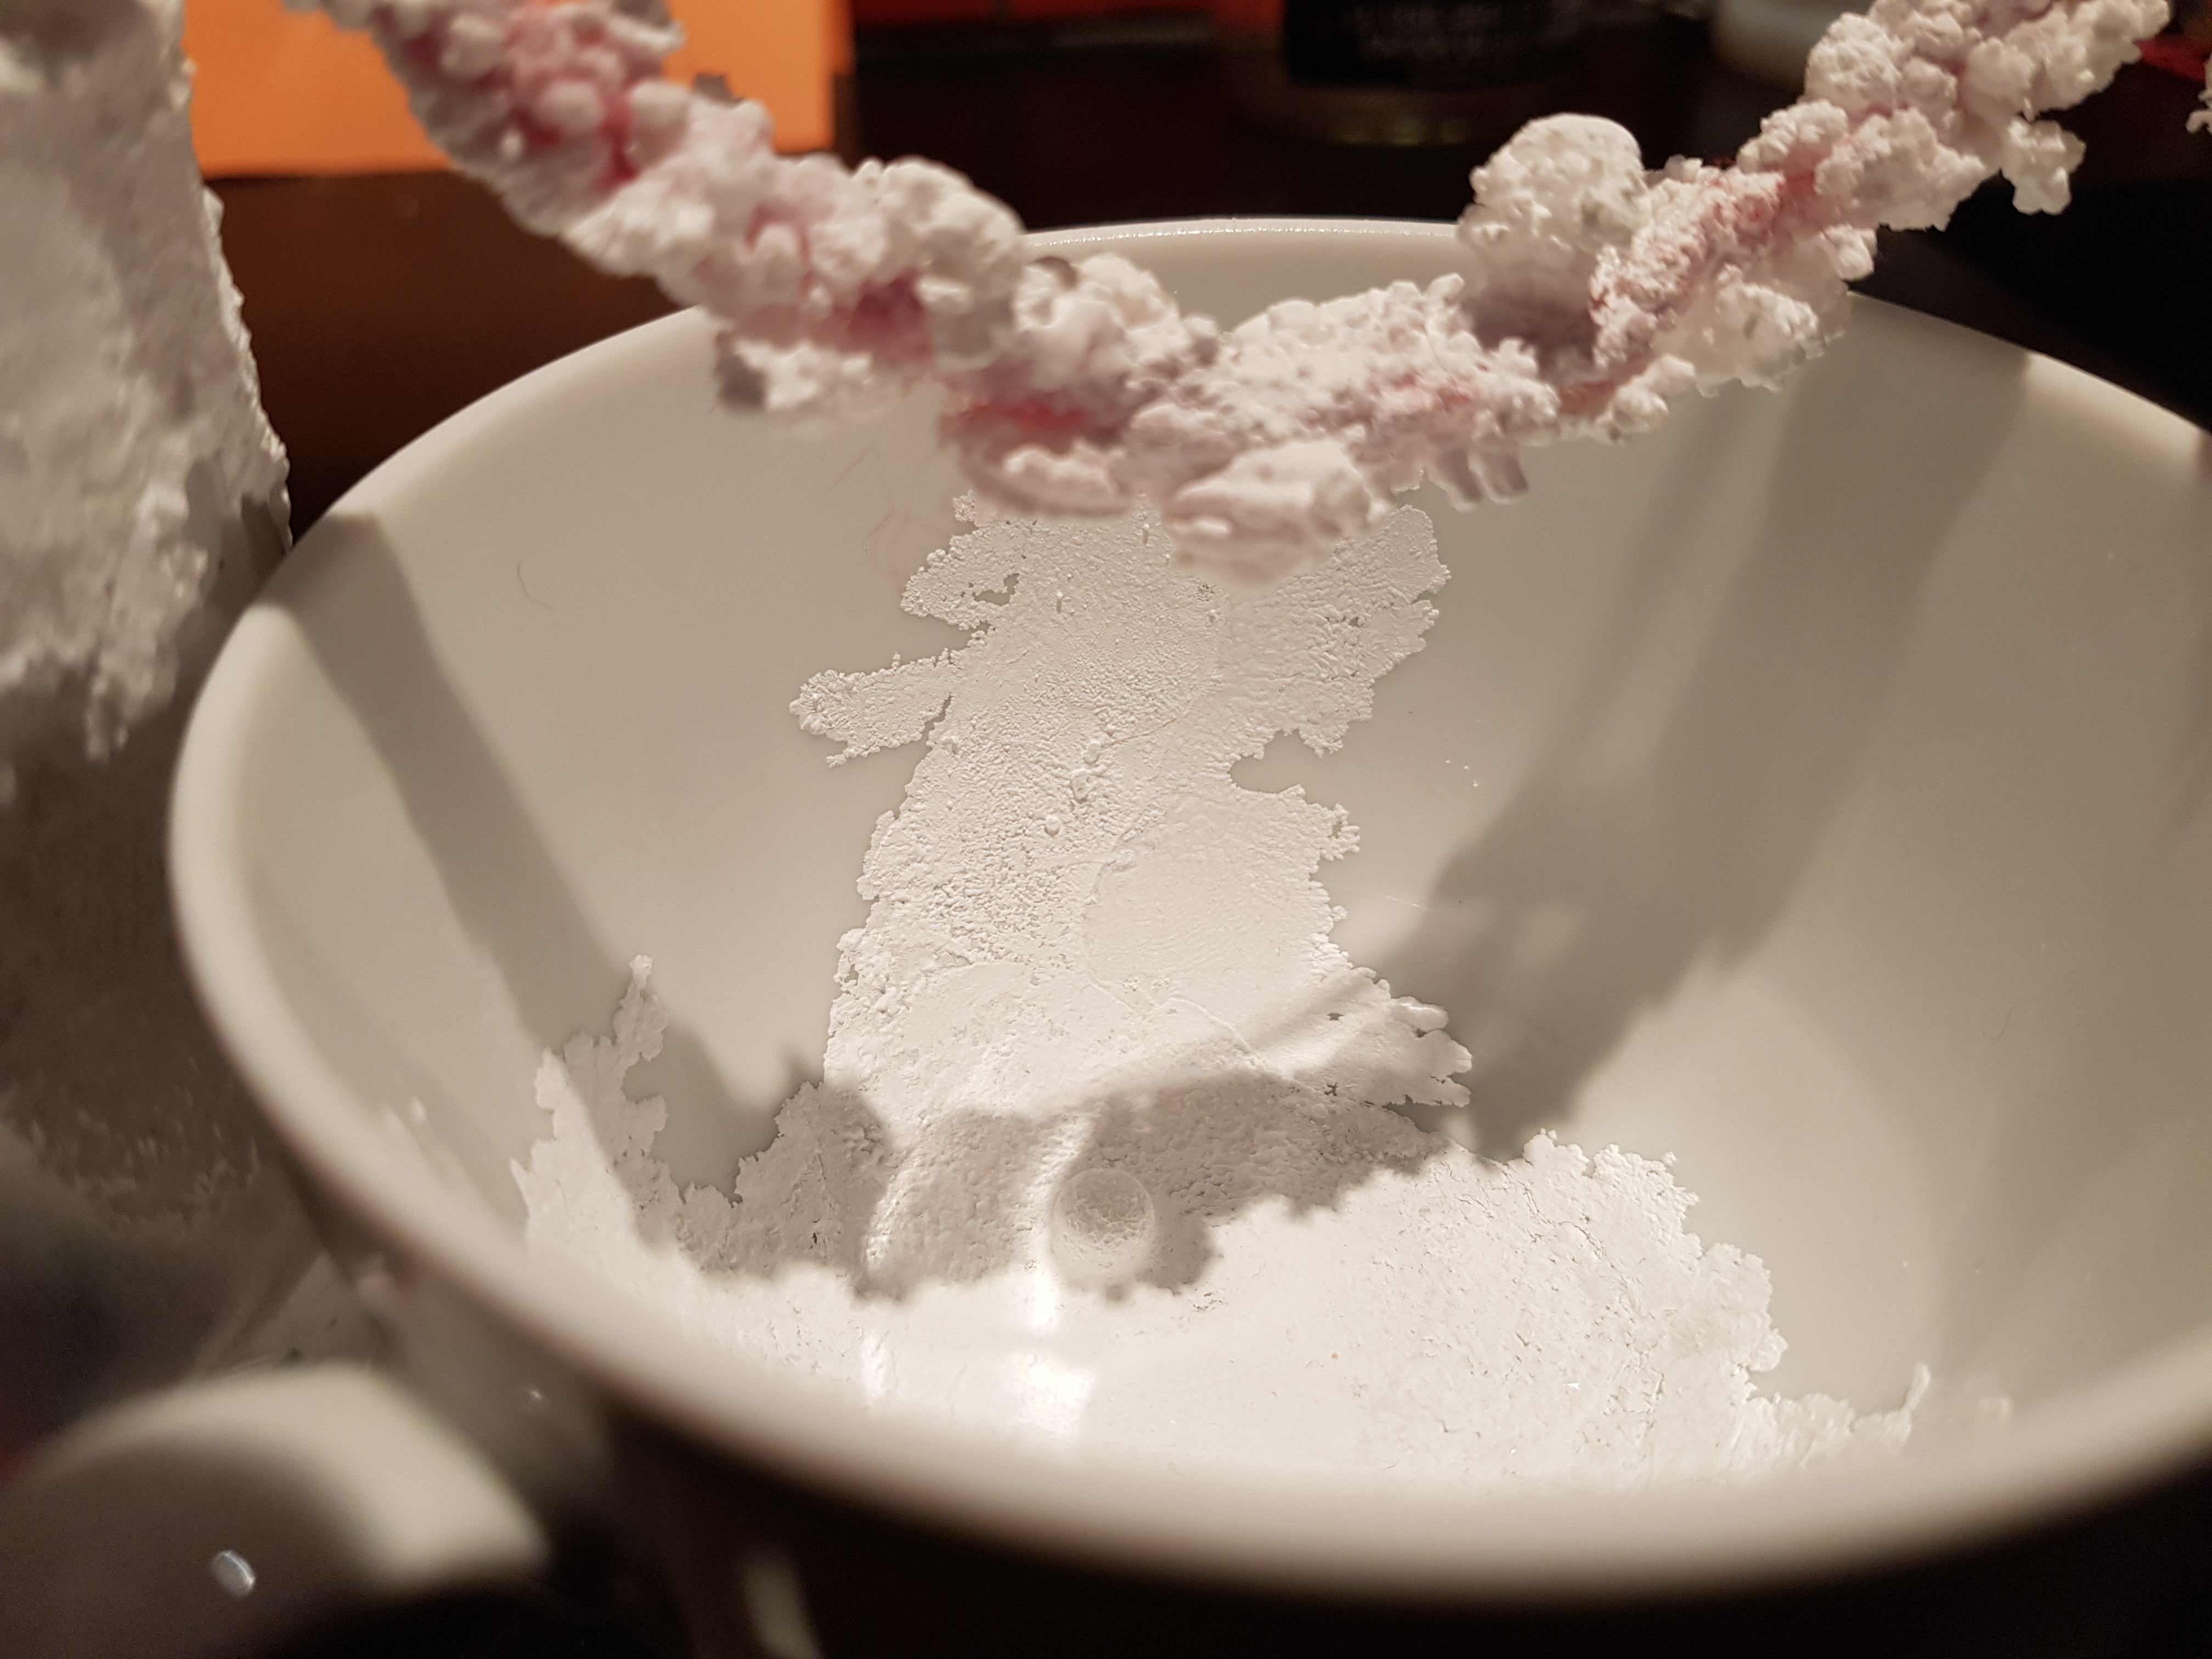
\includegraphics[scale=0.08]{LateX/Images/stalactitestalagmite.jpg}
  \caption{stalagctite and stalagmite}
\end{figure}
~\\[1cm]
~\par
However, the inside of the stalactite contains no hole, since the sodium bicarbonate was deposed around the rope, and not a plane. That is why we can not see any hole, but a zone where the water concentrates and evaporates. This water ``pushs'' the solid sodium bicarbonate. With time, the stalactite grows around the rope, in an uniform way, whereas the dripping follows an axis, during the formation of a stalactite inside a cave.
\\[1cm]
% insérer photo de l'intérieur du stalactite ET du stalagmite
  \begin{figure}[!ht]
      \begin{minipage}[c]{.46\linewidth}
          \centering
          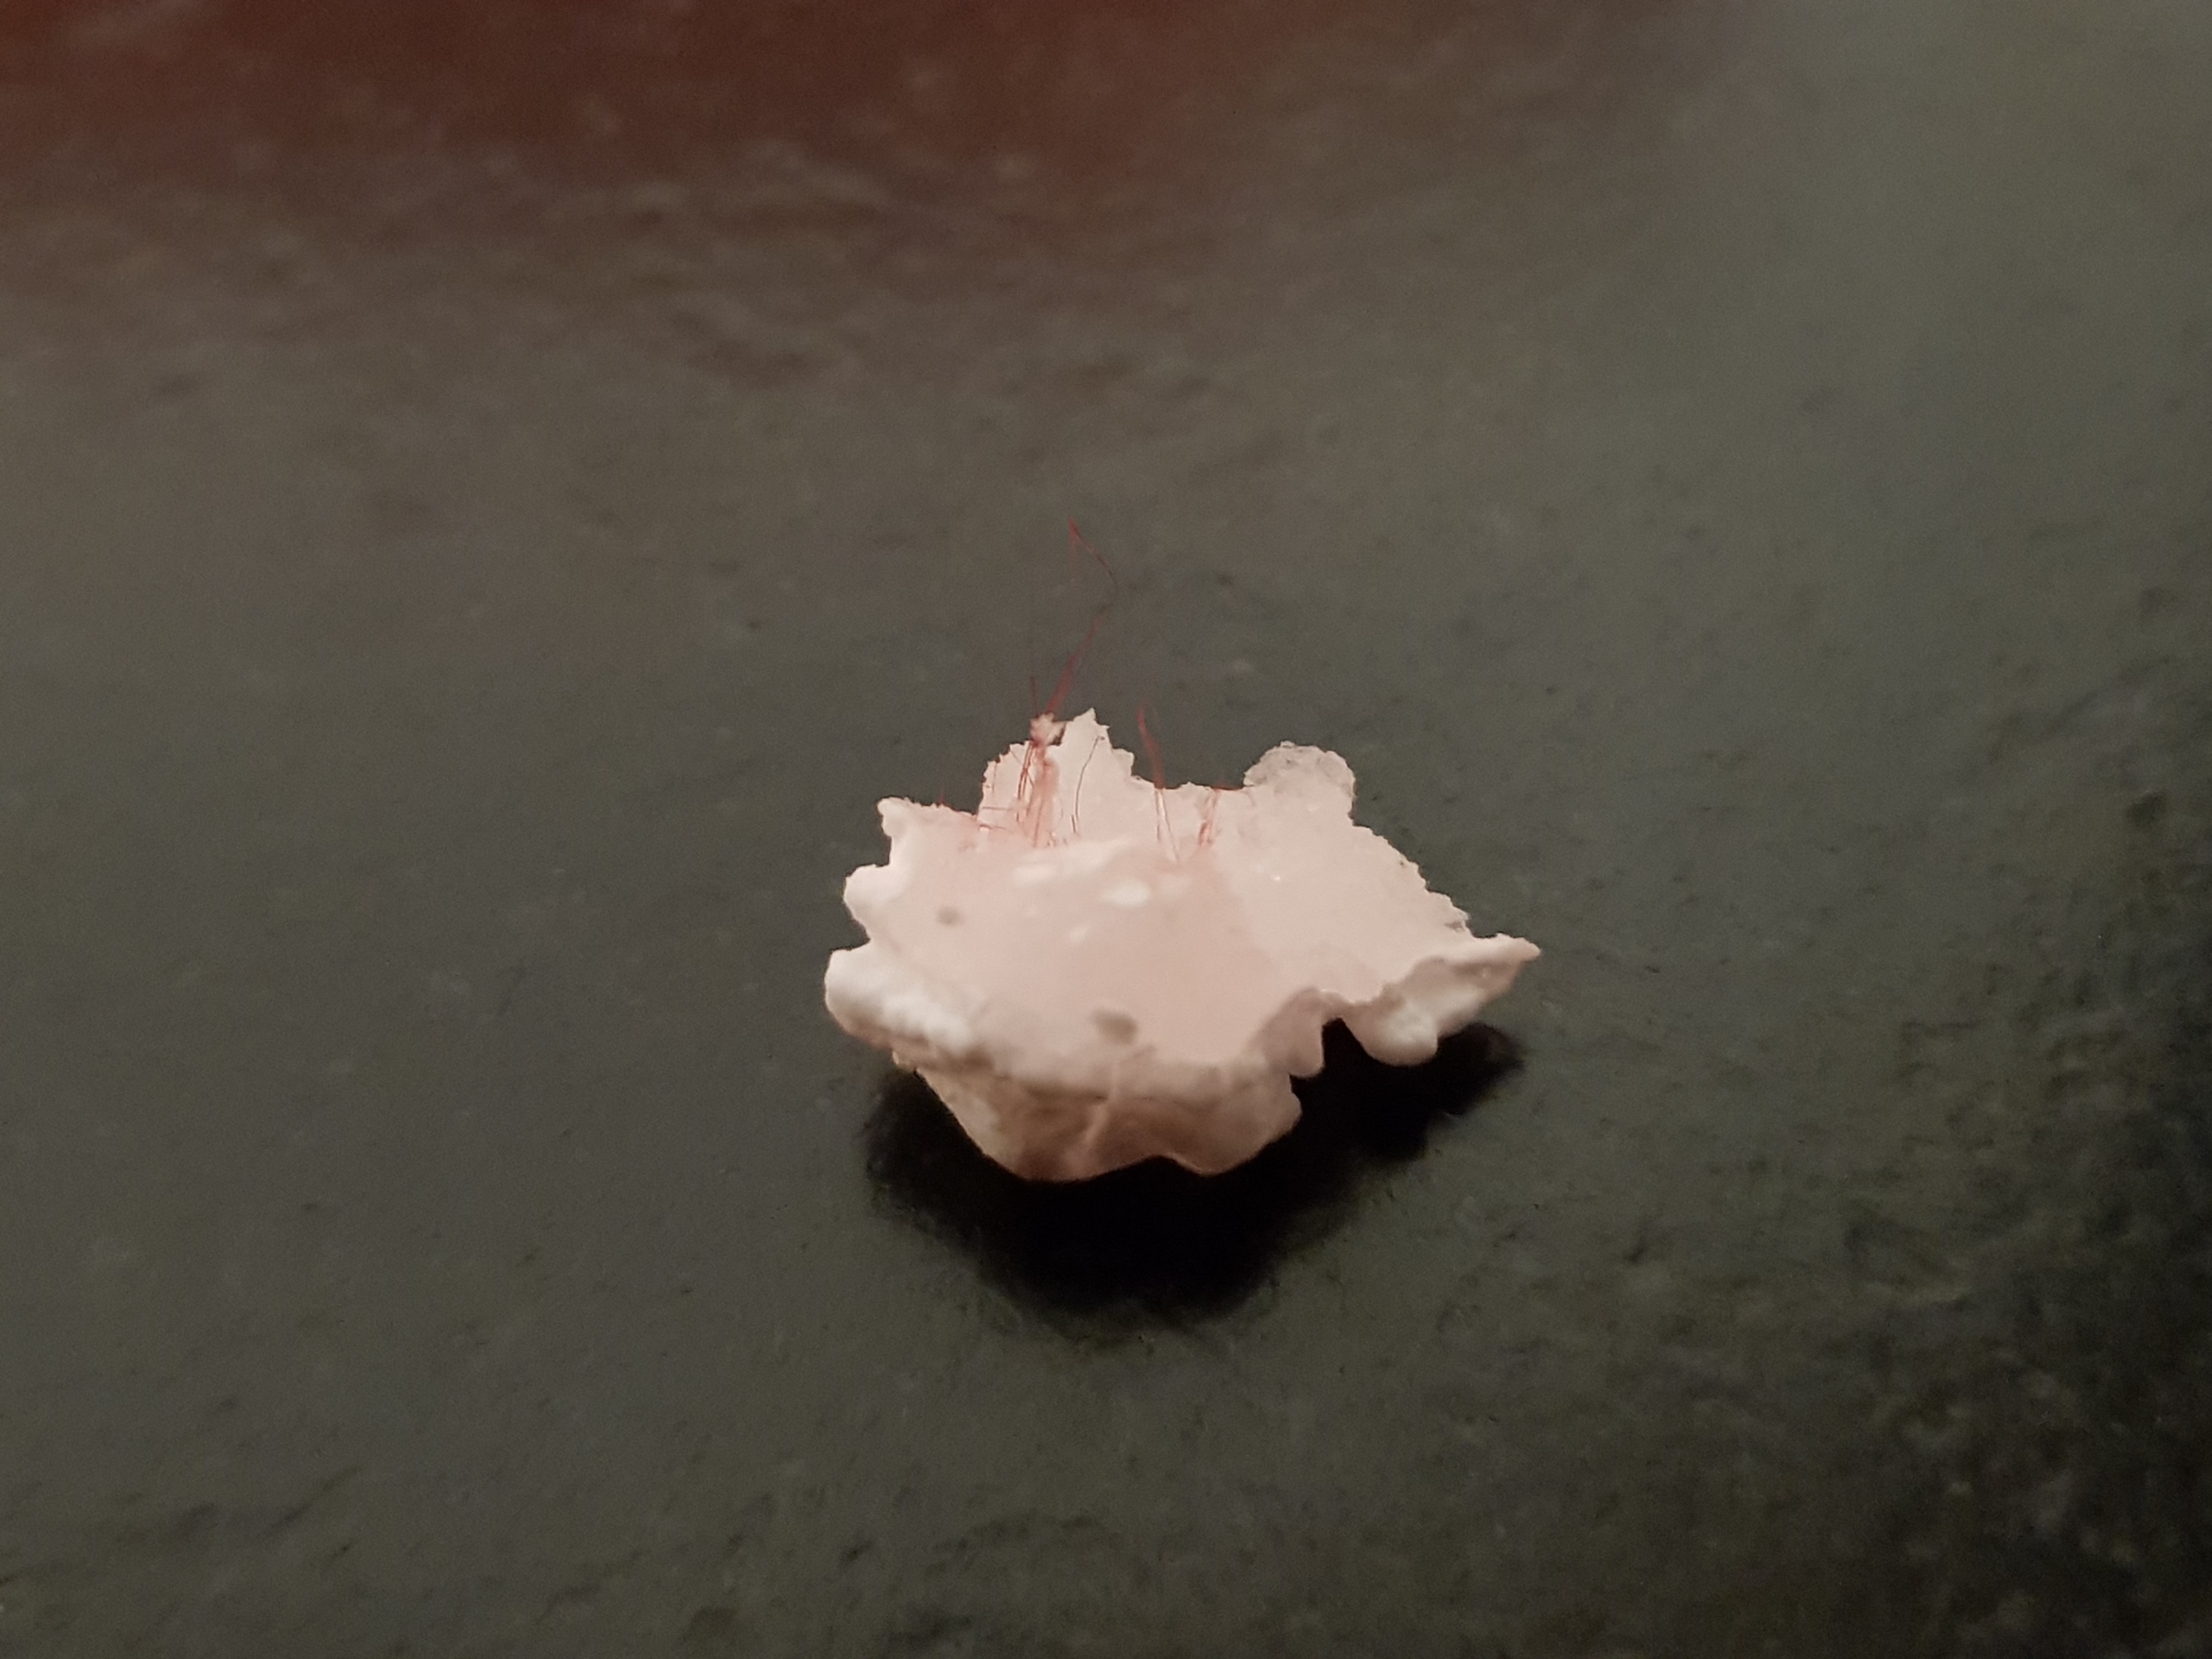
\includegraphics[scale=0.06]{LateX/Images/stalactiteslice.jpg}
          \caption{We can notice the solid zone, and at the center the zone that contains semi-liquid water saturated with sodium bicarbonate}
      \end{minipage}
      \hfill%
      \begin{minipage}[c]{.46\linewidth}
          \centering
          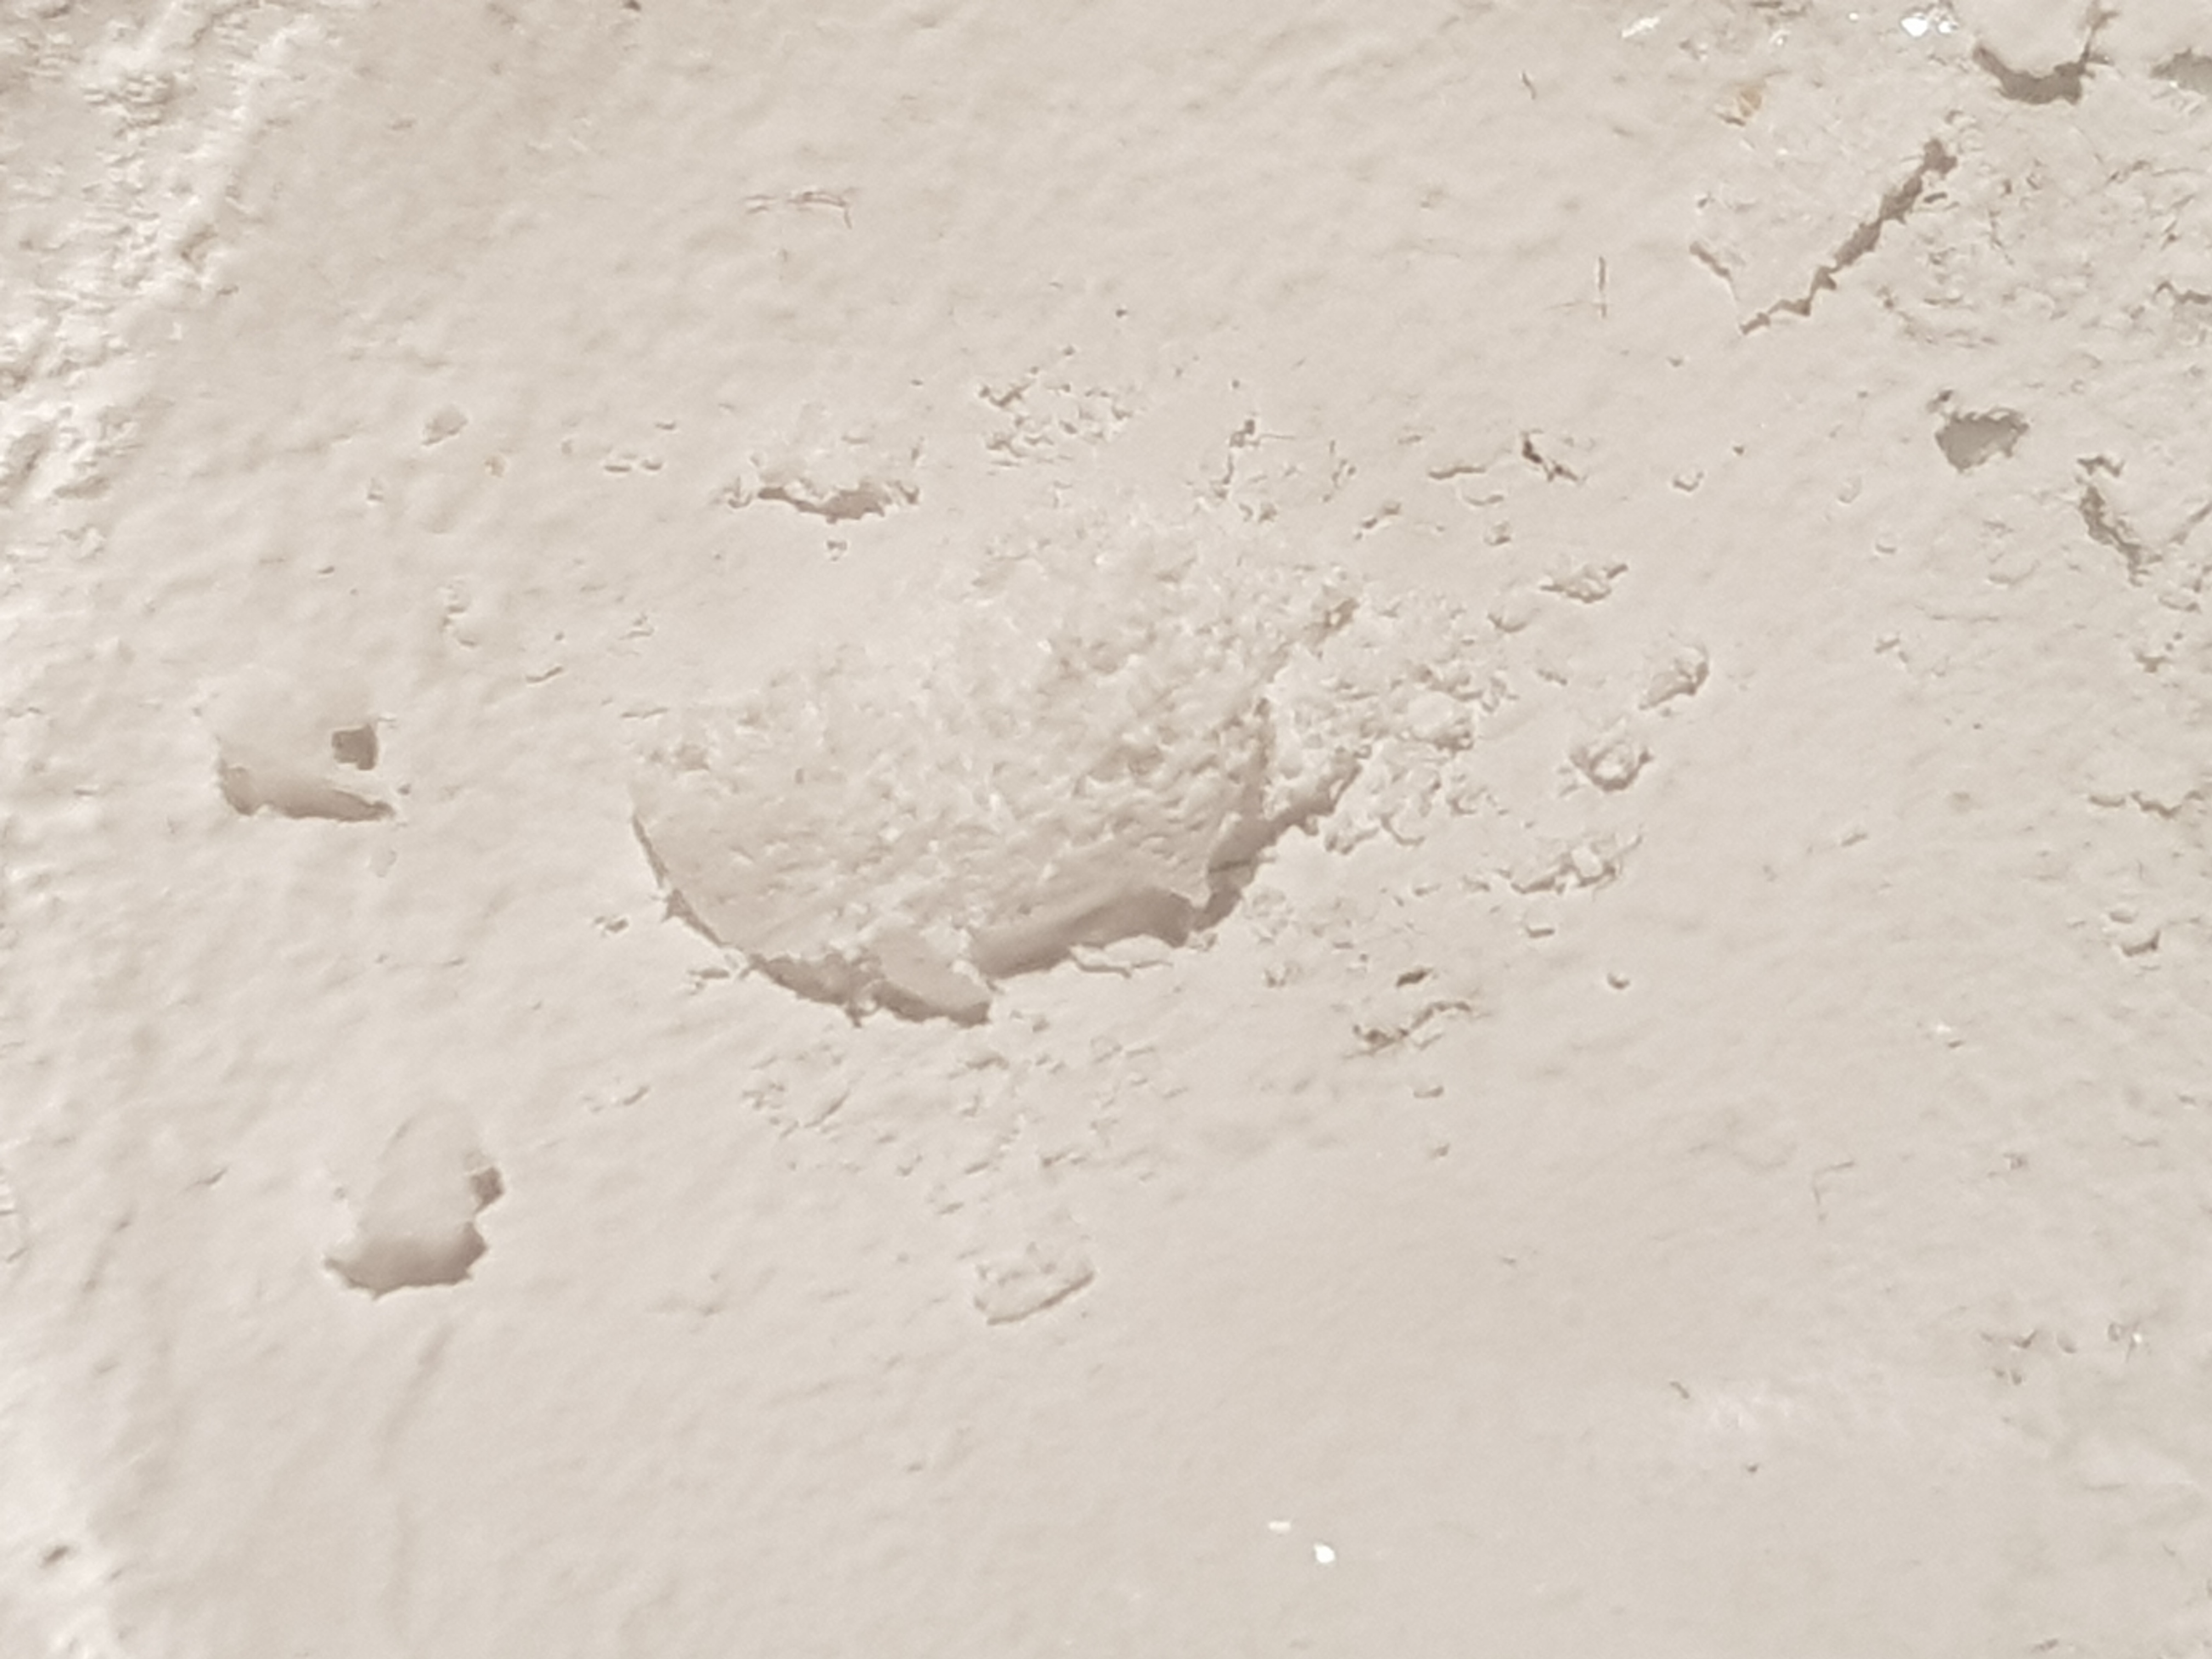
\includegraphics[scale=0.06]{LateX/Images/stalagmiteexp.jpg}
          \caption{The stalagmite is entirely solid, or more accurately it is composed of powder of sodium bicarbonate for its formation process is not the same as stalactites'one}
      \end{minipage}
    \end{figure}
% insérer le Qwer-Code
\begin{figure}[!ht]
  \centering
  
\includegraphics[scale=1]{LateX/Images/frame.png}
  \caption{QR Code leading to the link of a video that shows the evolution of the experiment}
\end{figure}
\clearpage

\chapter{Gravitational flow speleothems : flowstone, draperies, rimstone}
~\par
Once water reaches  a cave, gravity makes it flow toward the water table.  On its way there, it will give up most of its mineral load, generating a variety of speleothems. Flowstone forms wherever water flows in thin films (laminarflow) over a larger area, usually starting on a wall and continuing on the floor.\\
\begin{figure}[!ht]
  \begin{minipage}[c]{0.50\linewidth}
    \centering
    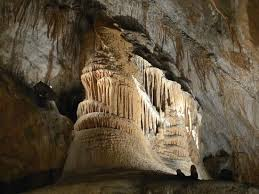
\includegraphics[scale=0.8]{LateX/Images/flowstone.jpg}
    \caption{Photography flowstone inside the cave of Mole Creek\cite{flowstone}}
  \end{minipage}\hfill%
  \begin{minipage}[c]{0.50\linewidth}
    \centering
    \includegraphics[scale=0.2]{LateX/Images/draperies.jpg}
    \caption{Draperies inside the cave of Fontrabiouse}
  \end{minipage}
\end{figure}
\clearpage

Draperies form on the ceilings and walls as thin sheets with the appearance of curtains, sometimes smooth, sometimes wavy. When thin, translucent, and with colored bands in them, some peoples call them ``bacon'' because of the striking resemblance to that popular food item.\\

They are actually formed by the same process than the stalactites. However, in this case, they do not drip vertically, but following the curve of a wall.\\
\begin{figure}[!ht]
  \centering
  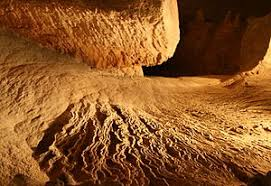
\includegraphics[scale=1]{LateX/Images/rimstone.jpg}
  \caption{Rimstone in the Endless Caverns, Virginia, USA\cite{caverimstone}}
\end{figure}


Rimstone precipitates on the rim of overflowing pools, initially as a thin blade that in time may grow into a solid dam up to 12 feet high. Rimstone pools form behind such dams.\\

\chapter{Capillary flow speleothems : shields, cave coral (popcorn), eccentrics}
~\par
When water flows through one very narrow (less than millimeter wide) conduits, it can sometimes defy gravity and flow upward, because of the high pressure inside those conduits. The mineral load it carries can be deposited (precipitated) into all sorts of surprising speleothems. Shields are in a way a very special of draperie. Two semicircular plates start growing parallel to each other on the left and right sides of a narrow (capillary) crack. They can grow in any direction but the most striking are the ones that grow steeply upward. Shields can reach more than three feet in diameter and eventually water starts flowing over their edge, the plate (tubular) growth becoming a normal flowstone growth, so that the shield often looks like a fringed canopy.\\
\begin{figure}[!ht]
    \centering
    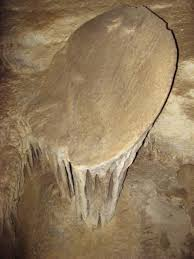
\includegraphics[scale=0.8]{LateX/Images/shield.jpg}
    \caption{Shield inside the Lehman Cave\cite{caveshelder}}
\end{figure}
\clearpage
Cave coral (popcorn in North-America) are essentially globular individual or clustered speleothems that may ressemble coral or grapes.
Their origin is not well understood and there are several theories regarding their formation. It is most probable, though, that capillary flow is involved.\\
\begin{figure}[!ht]
  \centering
  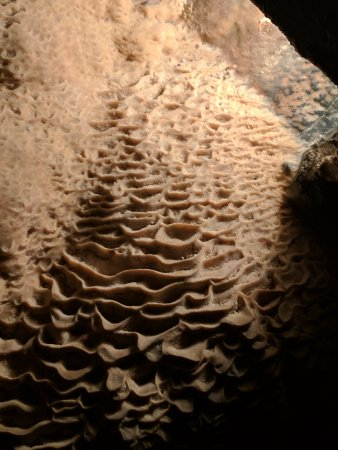
\includegraphics[scale=0.5]{LateX/Images/coral.jpg}
  \caption{Photography of cave coral\cite{cavecoral}}
\end{figure}
Eccentrics are by far the most spectacular and admired speleothems. They are made of very pure calcite crystals growing « eccentrically » (i.e., in any spatial direction), often against gravity. When growing from stalactites (or ceiling and wall) they are called helictites ; when growing from stalagmites (and floor) they are called heligmites. Though capillary flow is again most probably involved, exactly how remains a mystery to this day. Emil Silvestru's researches has suggested that natural electrical charges may also be involved.\\
\begin{figure}[!ht]
  \centering
  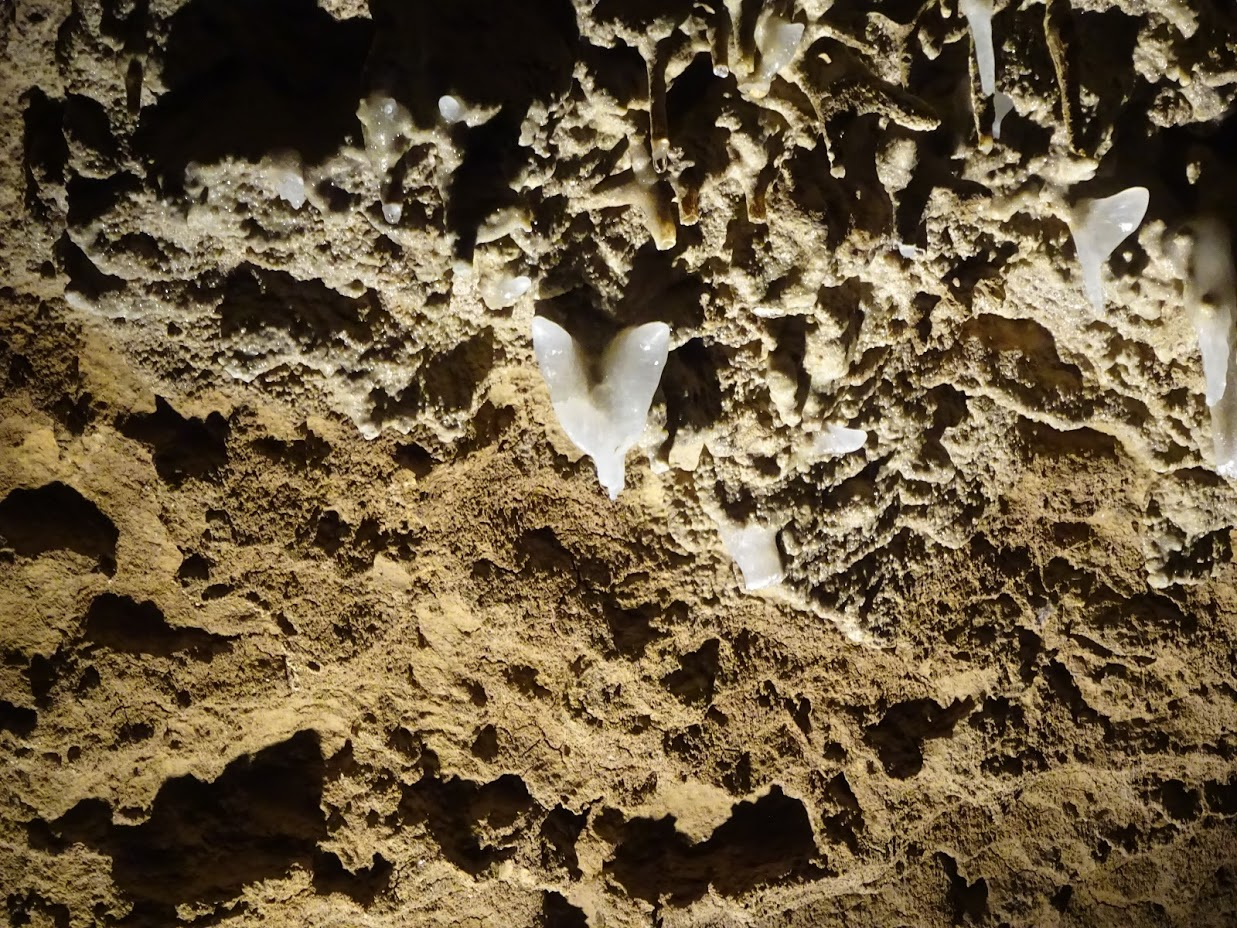
\includegraphics[scale=0.2]{LateX/Images/angel.jpg}
  \caption{heligmites, called also poetically ``Cave Angel''}
\end{figure}
\chapter{Pool speleothems : spars, shelfstone, cave (calcite) raft, cave pearls}
~\par
Oftentimes, the water that infiltrates caves accumulates in pools. Whenever that water is saturated  in calcite, wonderful things start happening. The walls become covered with large dogtooth spar calcite crystals. If there are some stalactites reaching the pools, their submerged parts will be covered with the same spar. The same phenomenon happens with the submerged parts of stalagmites. Sometimes the rims of the pools are lined with shelfstone, horizontal ledges of calcite always marking the surface of the water. When pool water is saturated and also very calm (no water dripping into it from above), thin flakes of calcite start growing, floating on the water – hence their name, cave rafts. When they become too heavy, they sink in the bottom of the ponds where they can accumulate in quite thick layers.\\
\begin{figure}[!ht]
  \centering
  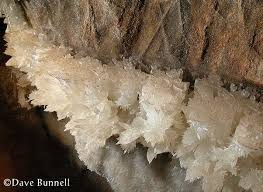
\includegraphics[scale=1]{LateX/Images/spars.jpg}
  \caption{Photography of cave spars\cite{cavespars}}
\end{figure}
\clearpage
The most spectacular examples of pool speleothems are cave pearls. They usually grow in shallow pools, layer after layer of smooth calcite or aragonite over all sorts of fragments like sand grains, chips of limestone, etc. Some of them are nearly spherical, some more or less irregular, and there are even polygonal ones (with angular facets). Their formation is only partially understood, especially the reason for their sphericity, since they lie on the bottom. Various scenarios of periodic rolling have been suggested, but none has been yet confirmed.\\
\begin{figure}[!ht]
  \centering
  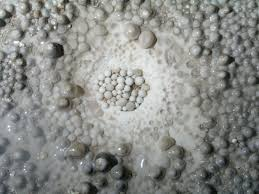
\includegraphics[scale=1]{LateX/Images/pearl.jpg}
  \caption{Photography of cave pearl\cite{cavepearl}}
\end{figure}

\chapter{The stuff in cave}
~\par
Caves are often thought of as little more than empty holes in the ground, but this is only half true; they’re holes with things within. Far from being just a hollow space, caves are full of curiosities – unusual rock formations, prehistoric artwork and, frequently, men who need rescuing.
Here are some things you can find in a cave.
\section{Crystal}
~\par
Scottish geologist Iain Stewart says that we know more about the outer edges of the solar system than we do about the Earth’s crust. This is a bit provocative, however, but the TV professor is right to think that there are some unexpected things hidden beneath our feet. Discovered by accident in 2000, Mexico’s Cueva de los Cristales (cave of the crystals) is one of our planet’s most amazing underground sights.\\
The miners who first discovered the cave must’ve been delighted – either they were going to be very rich or they were about to meet Superman. Sadly for the excited Mexicans, however, they were wrong on both counts. The crystals are made of gypsum and, despite being up to 12 metres long, are worthless compared to the lead and silver being mined nearby. But the problem is that the cave will be flooded and the crystals will be lost again, because the process of formation of this huge cristals is not compatible with a tourist activity.\\

\section{Lakes}
~\par
Most caves are wet – a bit damp, at least – but relatively few contain a whole lake. One of the most impressive cave lake is the Melissani Cave on the Greek island of Kefalonia.\\
Visitors can visit the two chambers of the Melissani Cave by boat. In the first chamber, some part of the ceiling has collapsed, allowing the sun to reflect in the clear blue water. This illuminates the lake and fills the cave with light, which is very unusual. The second chamber remains covered and, although not as visually stunning, the shade beneath the rock  allows to rest in the cool after the sunbath in the first chamber.\\
These lakes are formed by the dripping of water through the ceiling during millions of years. They are often really pure, for all the impurities are trapped in the ground up to the cave.
\begin{figure}[!ht]
  \centering
  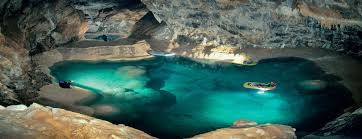
\includegraphics[scale=1]{LateX/Images/lake.jpg}
  \caption{Photography of the lake Achaïa\cite{lakeincave}}
\end{figure}
\section{Paintings}
~\par
Cueva de las Manos, in Argentina, has handprints on the wall that are between 9,500 and 13,000 years old. The images are stenciled outlines, made by placing one hand on the wall then blowing colour around it. Somehow this technique makes the pictures seem more three dimensional – it is easy to visualize a caveman’s hand in the space left behind, pushed against the wall as he made one of these basic self-portraits.\\
Analysis of the hands suggests that they are mostly from teenage boys, possibly created as part of a coming of age ritual. There are also some outlines of the feet of American Ostriches, made using the same technique. These are not the only type of paintings in the cave. Cueva de las Manos also has drawings of animals and hunting scenes, like some other caves around the world. Experts believe that these were not made just for decoration, but as messages for other people.
\begin{figure}[!ht]
  \centering
  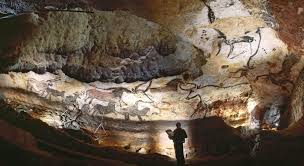
\includegraphics[scale=1]{LateX/Images/paintings.jpg}
  \caption{Photography of paintings in the cave of Lascaux in France\cite{cavepaintings}}
\end{figure}
\clearpage
\section{Rock salt}
~\par

The salt cave is lined with Himalayan rock salt boulders, and literally tons of granulated salt rest on the floor of the cave.\\

The Himalayan rock salt is millions of years old and it contains over 84 different minerals' traces which are readily absorbed by the human body.\\
Similar caves can be found all around the world. The Salzwelten salt mines in Hallein near Salzburg (Austria) is very famous in Europe.
As pure salt is diffused into the salt cave, the healing begins. Negative ions are released into the air, helping to promote calmness and toxins begin to be removed from the air which you breathe.\\

Some therapies consist of simply go and stay some hours inside the caves that contain those salts, in order to breathe more efficiently
\begin{figure}[!ht]
  \centering
  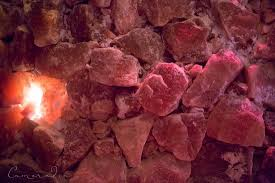
\includegraphics[scale=1]{LateX/Images/salt.jpg}
  \caption{Photography of some salt from a cave\cite{cavesalt}}
\end{figure}
\newpage
\chapter{Destructive speleology}
~\par
There are different impacts of the human activity in caves : the destructive speleology, the development and the pollution of the caves by water.
\begin{itemize}
  \item The speleology is the study of caves by exploration and scientific research. In order to explorate, speleologists destroy some parts of the rock to discover all the caves. But some people destroy parts of the rock in a cave completely explored or smear it. So the caves are destroyed in several place. Other people tag walls, littered garbage or break stalactites and stalagmites to take them as souvenirs.
  \begin{figure}[!ht]
      \begin{minipage}[c]{.46\linewidth}
          \centering
          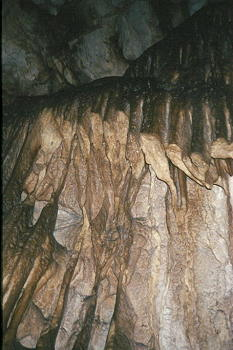
\includegraphics[scale=10]{LateX/Images/brokenstalactite.jpg}
          \caption{Stalactites broken in  the ``Trou de l'Eglise'' cave\cite{brokenstalactite}}
      \end{minipage}
      \hfill%
      \begin{minipage}[c]{.46\linewidth}
          \centering
          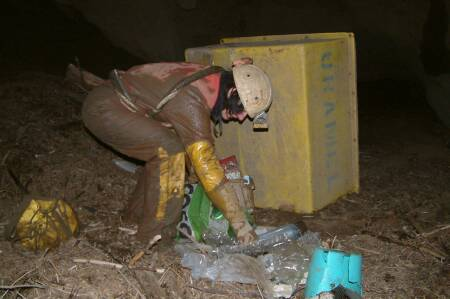
\includegraphics[scale=0.6]{LateX/Images/garbageincaves.jpg}
          \caption{Garbage in caves\cite{garbageincaves}}
      \end{minipage}
      \hfill%
      \begin{minipage}[c]{.46\linewidth}
          \centering
          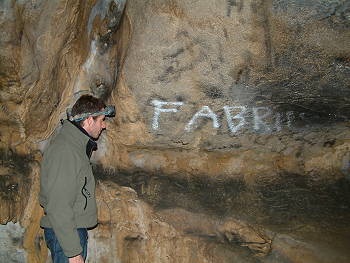
\includegraphics[scale=1]{LateX/Images/tagincaves.jpg}
          \caption{Tag in the ``Trou de la Louve'' cave \cite{tagincaves}}
      \end{minipage}
  \end{figure}
  \item For the accessibility and the comfort of the visitors, the caves are constructed. Stairs, cement walkways, bridge, lifts, security gates may be built to ease the accessibility to the caves. So the people cannot break the stalagmites for instance. But the building of infrastructure in caves cause the destruction of the cave. In order to make a cement walkways some stalagmites have to be broken. To build a bridge the support of this equipment has to destroyed. Stairs have to be fixed to be erected. The most important problem when structures are built is that many materials must be imported. Therefore building and adding equipments change the structure of the cave.
  \begin{figure}[!ht]
      \begin{minipage}[c]{.46\linewidth}
          \centering
          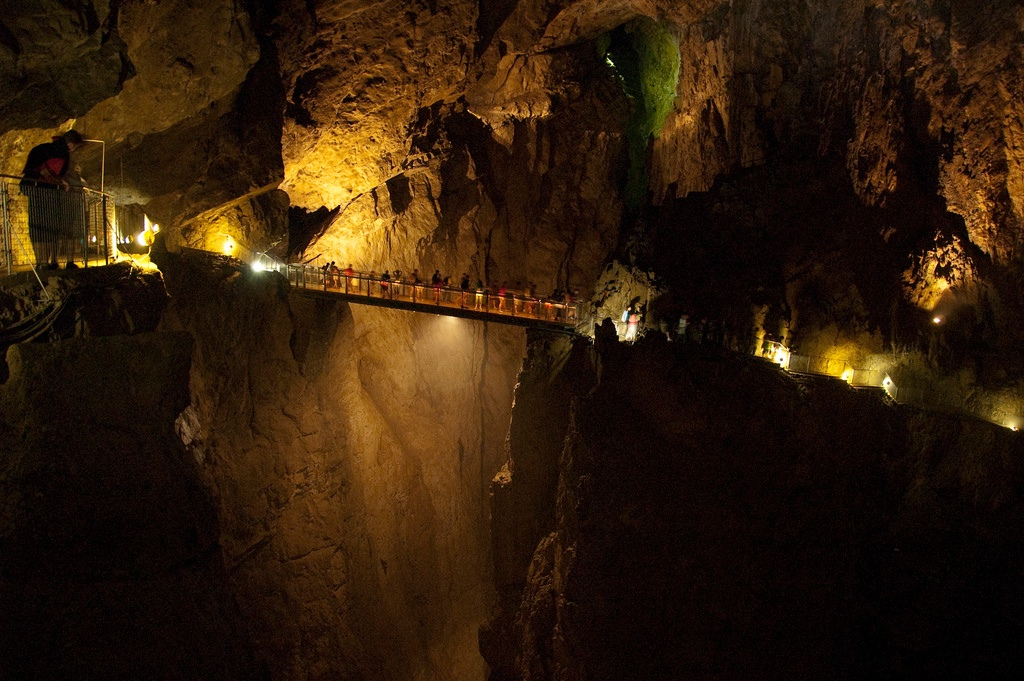
\includegraphics[scale=0.25]{LateX/Images/bridgeincaves.jpg}
          \caption{A bridge in the Skocjanske cave\cite{bridgeincaves}}
      \end{minipage}
      \hfill%
      \begin{minipage}[c]{.46\linewidth}
          \centering
          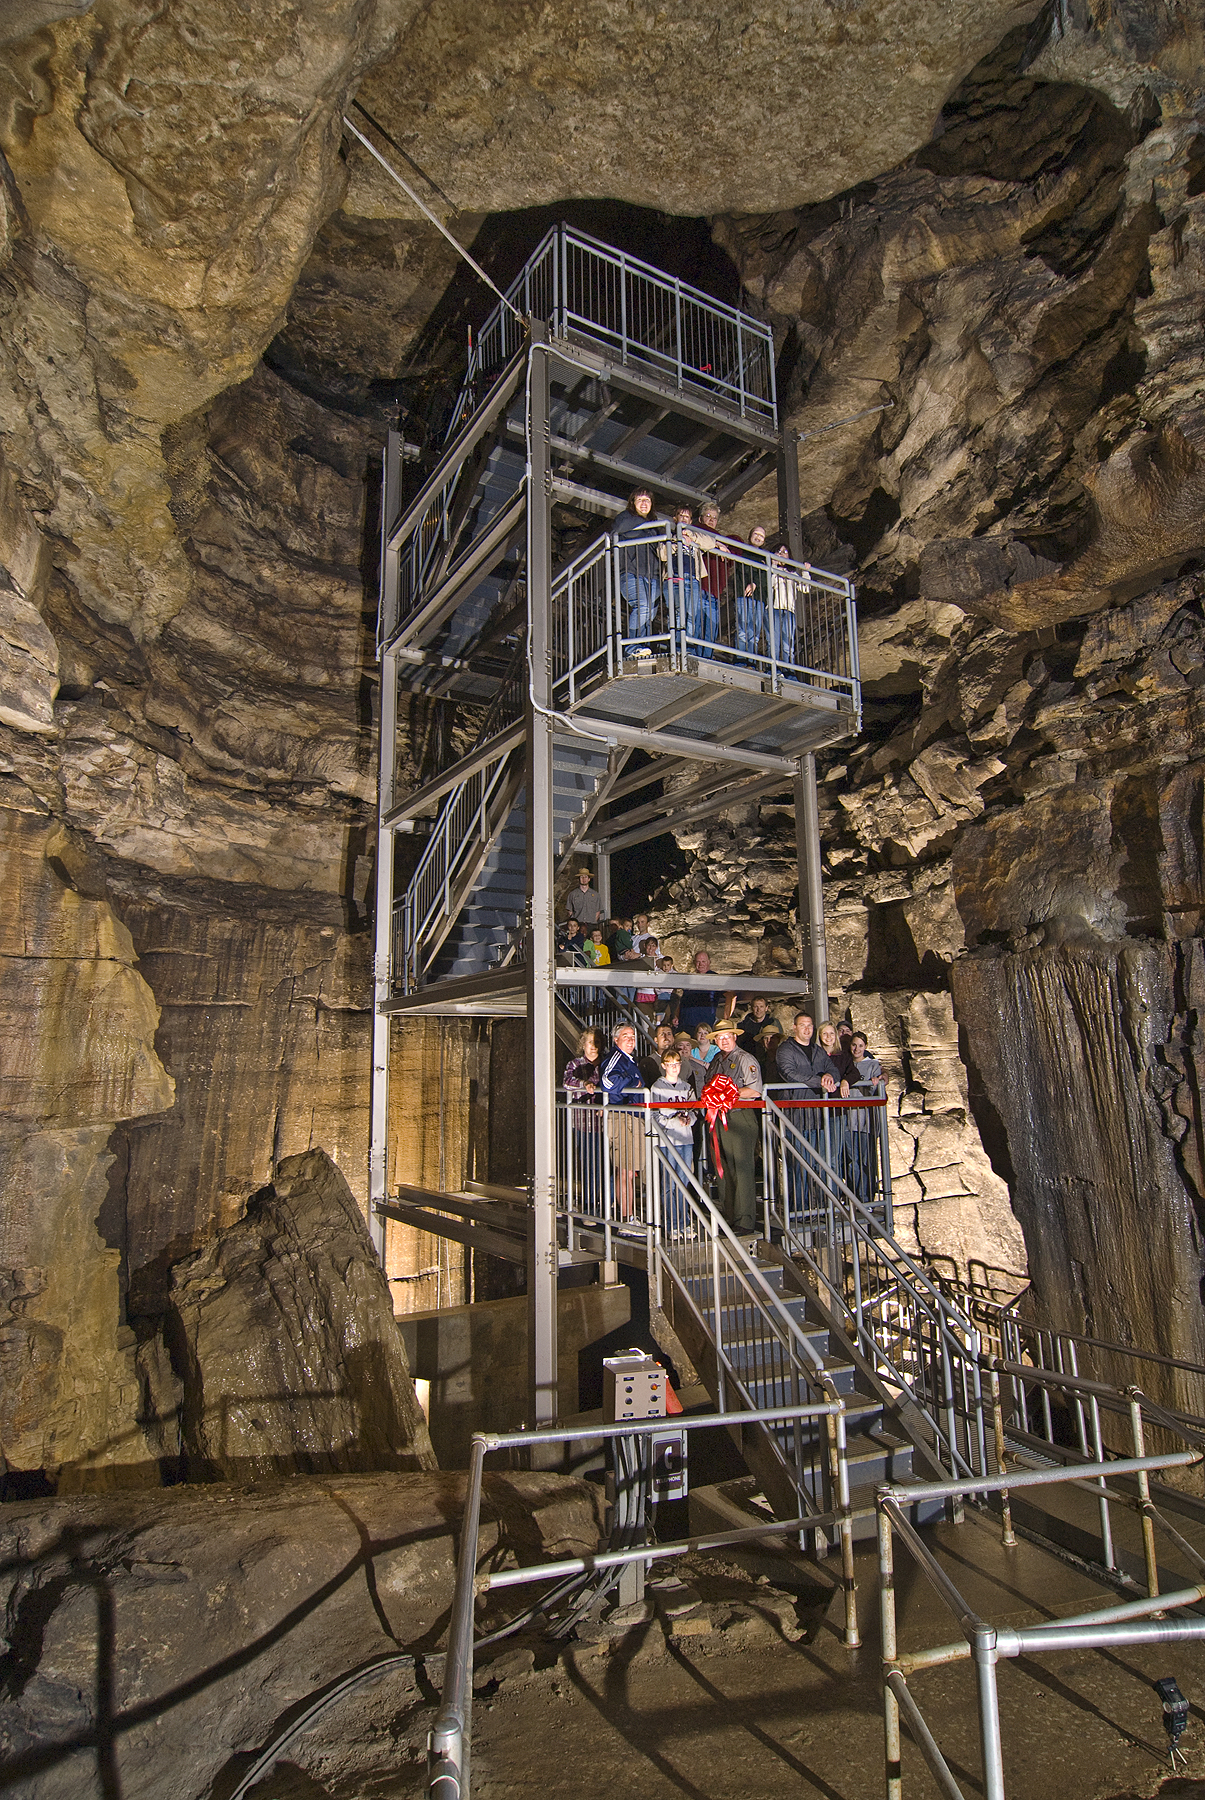
\includegraphics[scale=0.45]{LateX/Images/stairsincaves.jpg}
          \caption{Stairs in Mammoth Cave National Park\cite{stairsincaves}}
      \end{minipage}
      \hfill%
      \begin{minipage}[c]{.46\linewidth}
          \centering
          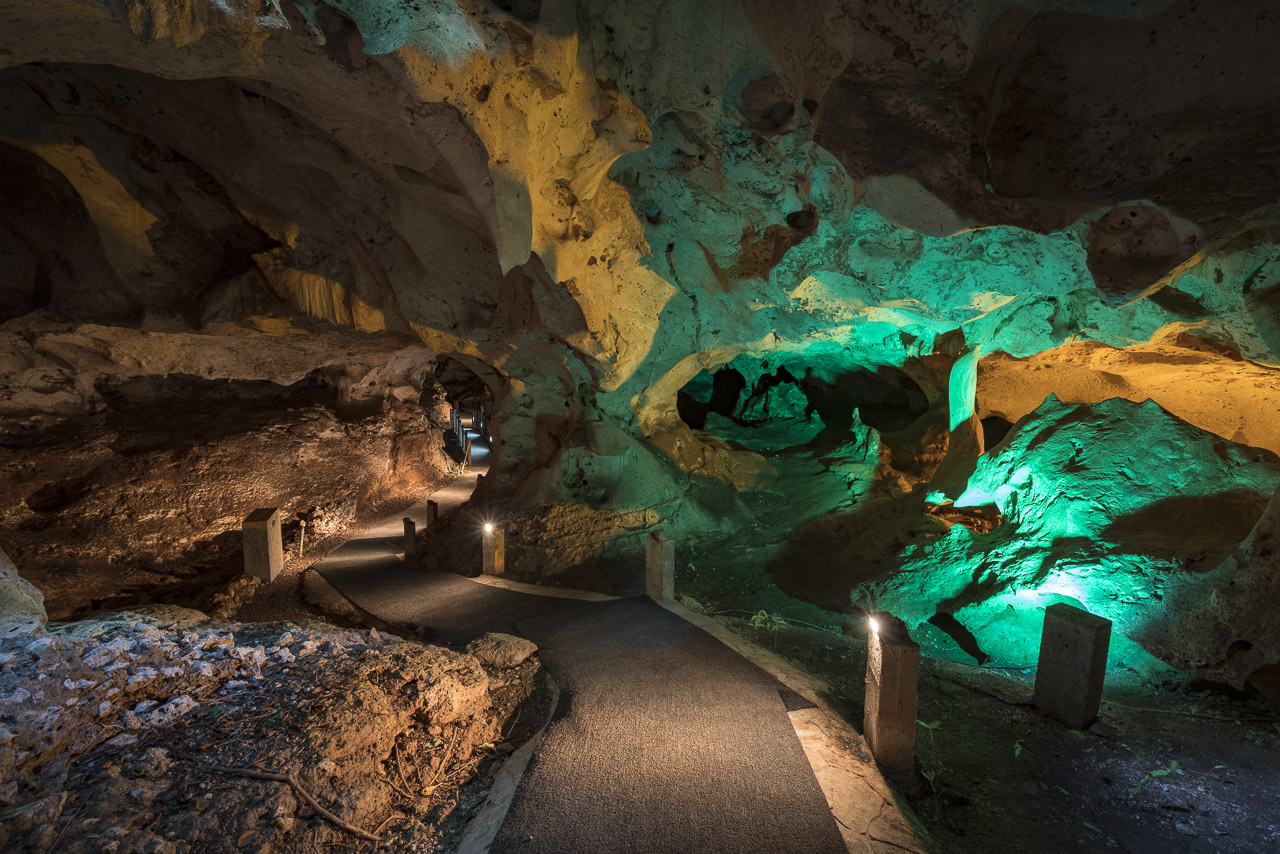
\includegraphics[scale=0.25]{LateX/Images/pathincaves.jpg}
          \caption{A path in Green Grotto cave\cite{pathincaves}}
      \end{minipage}
  \end{figure}
  \clearpage
  \item Human activities pollute the ground. In fact the surface water polluted infiltrates and go to the caves. The water is also polluted in the cave. In America, authority made classical sampling of fishes in the Bluestone River (river which separates the Virginia-West and the Virginia). After analysis, they discovered that there was a high concentration of polychlorinated biphenyls (or PCB), an industrial and dangerous compound. The authority searched the source of this problem.They found that the river water dripping into the cave was polluted by a chemical company using PCBs for its industrial operations. The water of this cave was polluted by human activity in surface.\\
  \newline
  \newline
  \newline
  \newline
  \newline
  \begin{figure}[!ht]
    \centering
    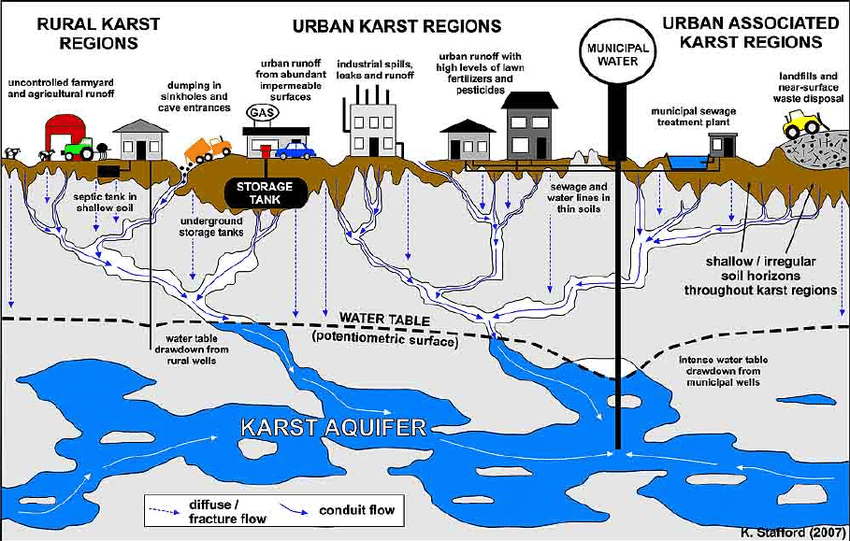
\includegraphics[scale=0.6]{LateX/Images/waterpollutionincaves.png}
    \caption{Scheme that explain the pollution of the water in caves due to the human activities in surface\cite{waterpollution}}
  \end{figure}

\end{itemize}
\newpage
\clearpage
\part{Biology}

\chapter{Cave’s conditions}
~\par
This chapter deals with the question of life in caves. It has been assumed for a long time that caves were almost empty, except rare specimens of fishes, small amphibians or mammals such as bats. However, we now know that reality is pretty different. We have yet discovered about 50,000 species of cave animals. And we are still discovering new ones regularly. For instance, in 2018, Chinese scientists discovered a cave beetle, whose has now the name of \emph{Xuedytes bellus}.
\smallbreak
To deal with cave’s species, we have first to talk about cave’s climatic conditions: when caves are long and deep enough, they are able to develop their own micro-climate. Dr Gheorghe Racoviță, a Romanian scientist has described three different micro-climates into the caves.

\begin{itemize}
  \item The \textbf{disturbance micro-climate}, or \textbf{entrance zone}, concerning the entrance of the cave, is characterized by numerous exchanges with the surface. For instance, the air fluctuation amplitude, with a temperate climate, is about 18.8°F (10°C), whereas it is usually of about 55.4°F (13°C). In this part of the cave, we can find green vegetation, because the luminosity rate is pretty high

  \item The \textbf{transitional micro-climate}, or \textbf{twilight zone}, concerns the part of the cave where the air fluctuation amplitude is less than 18.8°F (10°C) in temperate climate. Only a few resistant plants survive here.

  \item The \textbf{stability micro-climate}, called also \textbf{dark zone}, is the deeper zone of the cave, where the air fluctuation is reduced to less than 1,8°F(1°C), and where there is no more light.

\end{itemize}
\begin{figure}[!ht]
  \centering
  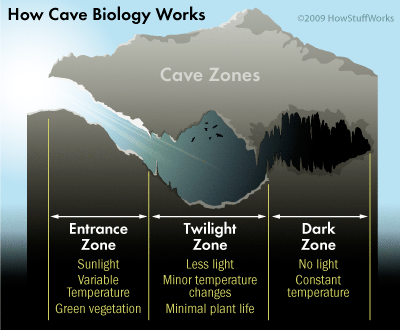
\includegraphics[scale=1]{LateX/Images/cavezones.png}
  \caption{The zones of the cave \cite{cavezones}}
  \label{CaveZones}
\end{figure}

\clearpage

We cannot define a precise average temperature of the caves. Indeed, this temperature depends of two factors. First, it depends of the cave’s location, and therefore of the atmosphere temperature. Then the temperature can vary with the depth of the cave. The heat of Earth plays actually a crucial role in cave’s climate. The average of these two factors determines the temperature of the cave. Usually, the caves are not located so deep. That’s why the temperature of the cave is often the same as the average temperature of the surface. The situation is the same in the case of the pressure in caves, which is about the same as the surface's one ($\simeq 1013 hPa$)
\smallbreak
However, cave humidity is really high, compared to the surface. For instance, the humidity rate is above 90 \% inside the caves, against about 70 \% in the region Languedoc-Roussillon, where the cave of Fontrabiouse is located.
\bigbreak
Even if describing air circulation in caves seems difficult, because of the variations due to the external air circulation, scientists reached to find three types of air displacements, or circulation. To obtain models, they used tracer gases such as $SF_{6}$ and $CCl_{2}F_{2}$ and determine their trajectory \footnote{Tracer gas: color and odorless gas, inert, non-toxic, that can’t displace air, and which is usually not present in the air and can,t be mistakable for other gases}. Here are the three different models of air-circulation that they obtained:
\begin{itemize}

  \item The \textbf{unidirectional (one-way) air circulation}. When a cave possesses only one entry, the warmer air, located deeper, rises up.  At the same time, the colder air flows in at the floor of the cave. This forms an air current. The deeper the cave is, the more powerful the air current is. This unidirectional air circulation can also cause the formation of “\textbf{cold traps}” . In temperate climate, during winter, the cooler air flows in the colder parts of the cave. Then, the rocks around become slowly colder. The rocks retain this coldness several 	months. Consequently, in summer, they are still cool when the water coming from the leaking ices outside flows into the cave. Finally, by being in contact with these cold rocks, water transforms into ice. That is why we can find huge ice formations in some caves, like in “The Mer de Glace” in France.

  \item The \textbf{bidirectional air circulation (two-ways)}. To have these kind of circulation, the cave must possess at least two entrances. Because of the difference of temperature between outside and inside the cave, air movements are created, particularly in Winter and Summer, when this difference is higher. Indeed, in Winter, the cold air comes into the cave by using the lower entry. Then, inside the cave, it warms up and rises up to go away at the upper entrance of the cave. In Summer, this process is inverted. \par
  Like in the case of the unidirectional air circulation, when the cave is located very high, the rocks of the lower part of the cave sustain the cold in Winter, and in Summer, when water flows, it turns into ice at this level. If these ice is perennial, that is to say if the ice is present in the cave all the year long, the cave is called a \textbf{dynamic ice cave}.

  \item The \textbf{multi-directional air circulation (numerous-ways)}. When caves possess many entrances, even little ones. Actually, the movements due to \textbf{chimney air flows} occurs. In winter, the warm air situated in caves leaves the cave. It is immediately replaced by colder air. In summer, this process occurs but is inverted, that is to say cold air leaves and warm air enters in the cave.

\end{itemize}

\begin{figure}[!ht]
  \centering
  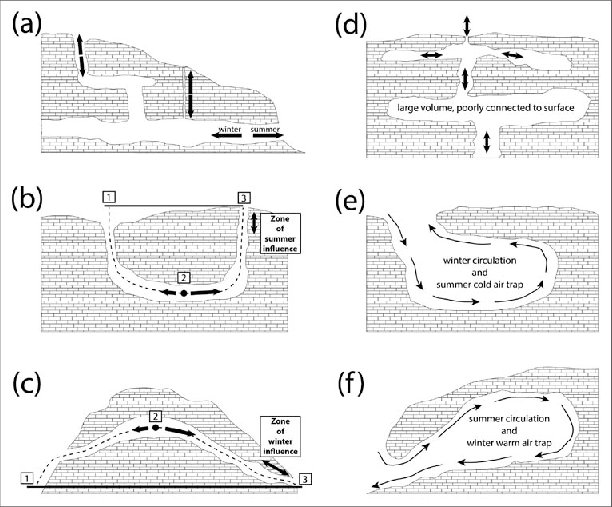
\includegraphics[scale=1.5]{LateX/Images/IllustrationsofmechanismsforcaveairflowForthermallydrivenflowsairflow.png}
  \caption{Aiflows in caves
    \\ a) and d) multi-directional air circulation
    \\ b) and c) unidirectional air circulation
    \\ e) and f) bidirectional air circulation \cite{caveaircirculation}\label{Airflows}}

\end{figure}

\clearpage

\chapter{life forms in caves: their physiology and behaviours}
~\par
As we have seen, the life conditions in caves are really hard. At first sight, life in the dark zone, the deepest and darkest part of the cave, seems very unlikely. However, life finds
always a way to develop itself. That is why many types of life forms can be found in caves. Four types have been defined:

\begin{itemize}

\item \textbf{Cavernicoles} are animals which live in dark environments, for instance caves. They are mainly arthropods, i.e. crustaceans, centipedes, millipedes, spiders, scorpions and insects.

\item \textbf{Troglophiles} (Greek for “who like caves”) are the animals that often live in dark environments, like caves, but are able to adapt themselves to live outside, in other environments with more light.

\item \textbf{Trogloxenes} (Greek for “foreign to caves") live only a part of their life cycle inside caves. They often go inside caves to sleep. These animals explore just the entry of the caves, where there is light. They are not particularly adapted to cave’s life, even if they can possess metabolisms that are also adapted for cave’s life (for instance echolocation). These animals are often the biggest in the cave. They include amphibians, small mammals like rats or bats. Humans, at the beginning of History were also trogloxenes.

\begin{figure}[H]
  \centering
  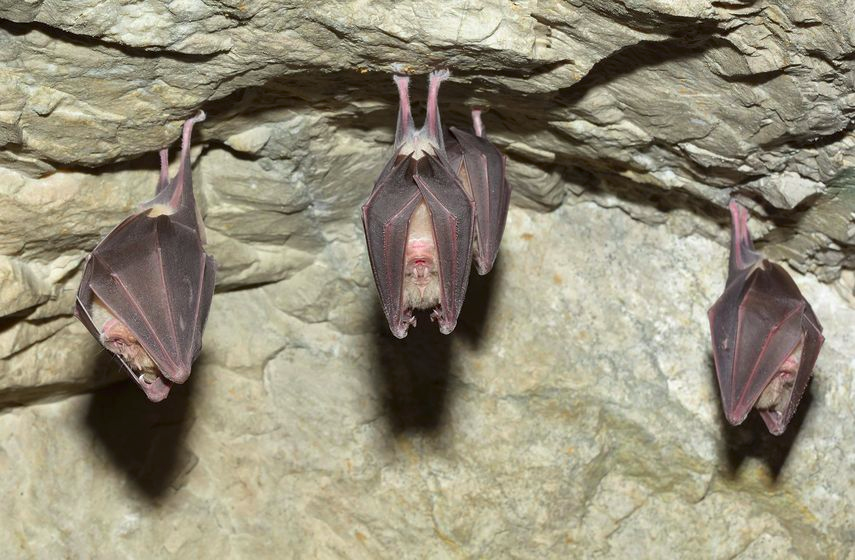
\includegraphics[scale=0.35]{LateX/Images/bats.png}
  \caption{Bats: troglophiles and trogloxenes \cite{batspresentation}}
\end{figure}

\item \textbf{Troglobites} (Greek for “cave dwellers”) have been living in the caves for a very long time. Therefore, they changed to adapt the hard conditions of life. These animals can not live outside cave’s environment. Troglobite species are often small amphibians or insects and arachnids like cave spiders or cave crickets and pseudoscorpions. We can also find centipedes, and even fishes that are troglobites. However, there are less troglobite predator species, probably because of the lack of food. This lack of food explains why the troglobite fishes are only located in tropical zones, for there are more organic matter, thus food in these areas.
\end{itemize}

\begin{figure}[H]
    \begin{minipage}[c]{.46\linewidth}
        \centering
        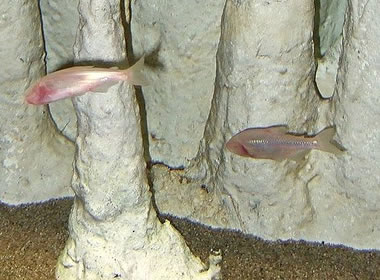
\includegraphics[scale=0.6]{LateX/Images/cavefish.png}
        \caption{Troglobite fish \cite{cavebeetle}}
    \end{minipage}
    \hfill%
    \begin{minipage}[c]{.46\linewidth}
        \centering
        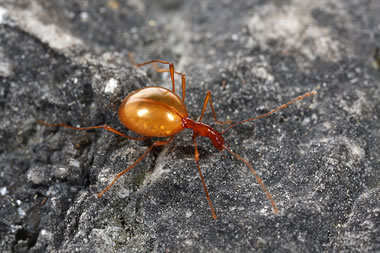
\includegraphics[scale=0.6]{LateX/Images/cavebeetle.png}
        \caption{Troglobite cave beetle \cite{cavefish}}
    \end{minipage}
\end{figure}

On Earth, troglobite insects or fishes are part the wildlife, though they constitute only a small part of it. Theses species would not indeed by their own go down into the caves. Now, how can they be all the same present in almost all the closed cave environments? The scientists have found some explanations. First, the animal could have migrated millions years ago, during the ice ages. They had indeed to find heat to survive. Consequently they went into the caves, and adapted themselves. When the ice age ended, they could not rise up to the surface, and were trapped into caves. Secondly, it can happen during summer, that when ice sheets melted, small animals are brought with water and fall into caves. However, the ice age do not explain the presence of troglobite species in the tropical area, since they were nearly not impacted by the glaciations. Some scientists suggest that some little fishes or animals lost their pigmentation or their eyes with time. Therefore, they migrated in caves to flee the light of the sun. Predators followed them, and that is why we can find an entire ecosystem even in tropical or sub-tropical areas.
\par
Cave’s organisms behave differently and have different physiology. This change is due to the high lack of food in caves, compared to the surface, and the limited size of the caves. Here are the main physiology’s differences between surface and cave-dwelling species:

\begin{itemize}
  \item \textbf{Higher lifetime}. Organisms in caves often have a very long lifetime, compared to similar surface-dwelling creatures. For instance, a 20-30 centimeter long salamander, called cave olm can live until 80 years. Surface-dwelling salamander can live a maxima 30 years in their natural environment.\par
  Now, this high lifetime is due to many causes:
  \begin{enumerate}
    \item An higher resistance against starvation, caused by the lack of food supplies compared to the surface.
    \item A modified metabolic rate , that is to say energy used by organism per unity of time.
    \item An altered circadian cycle(\ref{cyrcadiancycle1}), i.e. the different metabolisms higher rate per day. Caves’ organisms are not disturbed by many factors like luminosity, temperature, or humidity, because they are located in places with no changes: cave’s darkest zone. (can also be an absence of circadian cycle).
      \begin{figure}[!ht]
        \centering
        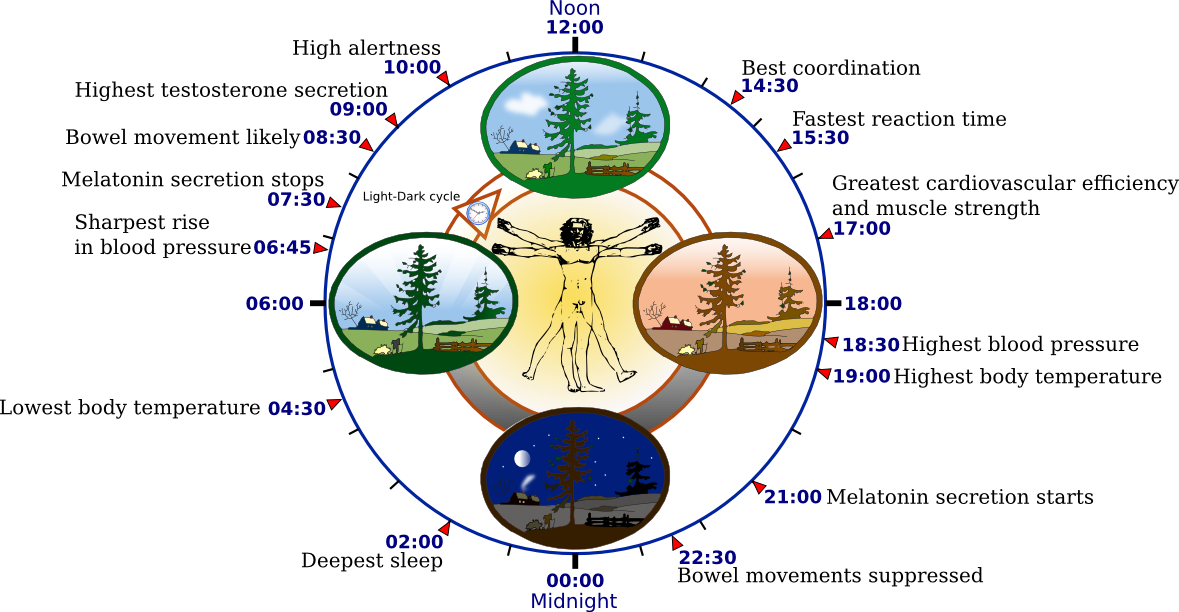
\includegraphics[scale = 0.4]{LateX/Images/CircadianCycle.png}
        \caption{Man circadian cycle \cite{circadiancycle}\label{cyrcadiancycle1}}
      \end{figure}
  \end{enumerate}
  \newpage
  \item \textbf{Lower fecondity}. Because of the lack of food, species like \emph{Troglohyphantes}, cave spiders, do not spawn as many eggs as surface-dwelling species (less than 10 eggs). However, the eggs of the troglobite spider are generally larger than phylogenetically close spiders'.
\end{itemize}

Besides, caves’ species behaviour are really different compared to other surface-dwelling species. Unfortunately, a few is known about cave’s organisms’ behaviours, because not a lot of observations were made. Many behaviours like reproduction, aggression, aggregation seem to be the same as the ones of surface-dwelling species.
\par
For spiders (like  \emph{LABIDOGNATHA Liocranidae Brachyanillus}, \emph{Liocranum and Agraecina}), we can notice a change. Indeed, this creature do still produce webs in caves but only to build a secured refuge. Webs are not used to chase. Spiders have to move in the cave to search preys.
\par
However, living in cave also reduce the adaptability of organisms to environments data (temperature, humidity, luminosity), because organisms are so well-adapted to their own cave’s conditions, that they can not support any change.

The human activity impacts a lot the life in caves. In fact, the artificial light, installed for visitors, change the conditions because they produce heat and the light disturbs species like the troglobxene bats. Moreover the presence of light in caves leads to the development of some new cave species, such as lampenflora. The $CO_{2}$ released by the visitors affect also the conditions of the cave.

\clearpage

\chapter{Food Chain}
~\par
As all  the ecosystems, inside the cave, we find predators and preys. This chapter deals with the cave food chain. \\
\par
At the bottom of the pyramid, we find mainly bacteria, often chemoautotrophic, heterotrophic and at the entry of the cave photothopic. We also find litter from the trogloxenes like bats’ guano and fungi. The chemoautotrophic bacteria produce their own organic matter by using chemical reactions. Heterotropics bacteria, such as \emph{Synechococcus elongatus} and \emph{Anacystis montana}  and fungi use rather readymade organic food molecules. Some Fungi like \emph{Armellia mellea}, \emph{Xylaria hypoxylon} and \emph{Xylaria polymorpha} or \emph{Poriaillanti} are wood-parasites, whereas \emph{Paecilomyces} grow on dead insects, and both \emph{Beauveria} and \emph{Hirsutella} develop on living insects, that they killed after feeding of insect’s organic matter. \\
\par
Then we find mainly arthropods and lot of troglobites creatures, which eat the fungi and the organic matter delivered by bacteria. Here there are mainly, millipedes (ex: \emph{Polydesmus angustus} or \emph{Brachydesmus superus}) or small crustaceans (ex: \emph{Niphargus fontanus}). \\
\par
The last level of the food chain pyramid is the predator’s one. Here we find the biggest animals like salamandres (ex: \emph{Eurycea lucifuga}), spiders (ex: \emph{LABIDOGNATHA Liocranidae Brachyanillus}, \emph{Liocranum} and \emph{Agraecina}), pseudoscorpions (ex: \emph{Roncus lubricus}), mites (ex: \emph{Calyptostoma velutinus}), fishes (ex: \emph{Astyanax jordani}) and also tiny poisonous animals like centipedes (ex:\emph{ Lithobius microps}). In Alpen we can find the strange \emph{cave olm}, which is the biggest predator of the caves where it lives. \\
\par
The main part of the trogloxenes chase outside from the caves, like bats.

\begin{figure}[!ht]
  \centering
  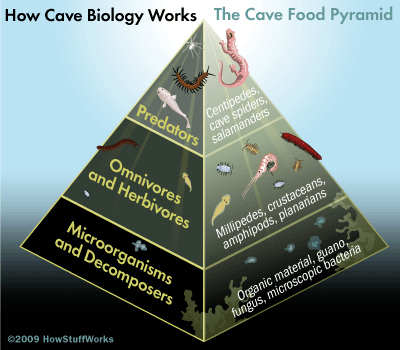
\includegraphics[scale=1]{LateX/Images/Foodchain.png}
  \caption{Cave's food chain \cite{foodchainpyramid}}
\end{figure}
\clearpage
\begin{figure}[!ht]
    \begin{minipage}[c]{.46\linewidth}
        \centering
        \includegraphics[scale=0.25]{LateX/Images/fnwickdavid.png}
        \caption{\emph{Lithobius microps}: a cave poisonous centipede\cite{fenwickdavid}}
    \end{minipage}
    \hfill%
    \begin{minipage}[c]{.46\linewidth}
        \centering
        \includegraphics[scale=0.25]{LateX/Images/cavefish2.png}
        \caption{\emph{Astyanax jordani}: a cave-dweller fish in Mexico\cite{rapsonandy}}
    \end{minipage}
\end{figure}
\begin{figure}[!ht]
    \begin{minipage}[c]{.46\linewidth}
        \centering
        \includegraphics[scale=0.25]{LateX/Images/calyptostoma.png}
        \caption{\emph{Calyptostoma velutinus}\cite{calyptostoma}}
    \end{minipage}
    \hfill%
    \begin{minipage}[c]{.46\linewidth}
        \centering
        \includegraphics[scale=0.25]{LateX/Images/salamander.jpg}
        \caption{\emph{Eurycea lucifuga}: a cave-dweller salamander\cite{cavesalamander}}
    \end{minipage}
    \hfill%
    \begin{minipage}[c]{.46\linewidth}
        \centering
        \includegraphics[scale=0.35]{LateX/Images/cavefungi.png}
        \caption{Fungi growing on a living insect\cite{cavesfungi}}
    \end{minipage}
    \hfill%
    \begin{minipage}[c]{.46\linewidth}
        \centering
        \includegraphics[scale=0.15]{LateX/Images/cavespider.png}
        \caption{\emph{Troglohyphantes}: a cave-dweller predator\cite{cavespider}}
    \end{minipage}
  \end{figure}

\clearpage

\chapter{Metabolisms}

\section{Bacteria metabolisms}
~\par
We will now focus on the different ways life found to develop itself into caves. We will start from the bottom of the food chain, meaning the bacteria specifics metabolisms. Then, we will see more accurately the specific features of trogloxene life. \\
\par
In caves, we find three types of bacteria: chemotrophic, heterotrophic and phototrophic, according to the part of the cave. They form the base of the food chain, thus the base of the entire cave ecosystem.\\
\par

\begin{figure}[!ht]
  \centering
  \includegraphics[scale=0.79]{LateX/Images/PhylogeneticTree.png}
  \caption{Bacteria phylogenetic tree\cite{phylobacteria}}
\end{figure}

First, what is the difference between them? Well, they do not use the same metabolism to survive. There are plenty of different variations of metabolism:\\
\par
\begin{itemize}
  \item \textbf{Photoautotrophs} are bacteria that can create their own organic matter with sunlight and mineral molecules. These organisms can be green plants or some bacteria. They possess organelle called chloroplasts, in which we can find chlorophylls. They use photosynthesis.\\
	The photosynthesis phenomenon occurs into chloroplasts. \\
  \begin{figure}[!ht]
    \centering
    \includegraphics[scale=0.3]{LateX/Images/Chloroplast.png}
    \caption{Scheme of a chloroplast:
              \\ 1. outer membrane
              \\ 2. intermembrane space
              \\ 3. inner membrane
              \\ 4. stroma
              \\ 5. thylakoid lumen (inside thylakoid)
              \\ 6. thylakoid membrane containing
	                \\ chlorophylle a
	                \\ chlorophylle b
		              \\ carotenoids
		              \\ xanthophylles
              \\ 7. granum (stack of thylakoids)
              \\ 8. lamella
              \\ 9. starch
              \\ 10. ribosomes
              \\ 11. DNA
              \\ 12. plastoglobule (lipid)\cite{chloroplast}}
  \end{figure}

  \begin{figure}[!ht]
      \begin{minipage}[c]{.46\linewidth}
          \centering
          \includegraphics[scale=0.15]{LateX/Images/AdenosineDiphosphate.png}
          \caption{Adenosine diphosphate\label{AdenosineDiphosphate}}
      \end{minipage}
      \hfill%
      \begin{minipage}[c]{.46\linewidth}
          \centering
          \includegraphics[scale=0.4]{LateX/Images/AdenosineTriphosphate.png}
          \caption{Adenosine triphosphate\label{AdenosineTriphosphate}}
      \end{minipage}
      \hfill%
      \begin{minipage}[c]{.46\linewidth}
          \centering
          \includegraphics[scale=0.5]{LateX/Images/InorganicPhosphate.png}
          \caption{Inorganic phosphate \label{InorganicPhosphate}}
      \end{minipage}
  \end{figure}
  Photosynthesis can be split in two main parts:
  \begin{enumerate}
    \item The \textbf{photochemical part} occurs inside thylakoids’ membrane. To arise, the cell or organism must be exposed to light and water. Besides, the cell has to possess ADP(\ref{AdenosineDiphosphate}), inorganic phosphate, noted “Pi”(\ref{InorganicPhosphate}) and an oxidizer, noted “R”. First, water comes through the roots to the leaves, inside the cells inside chloroplast. The photons, captured by the leaves cause chlorophyll's excitation, and the dissociation of water. Some of the atoms composing chlorophyll lose some electron.\\
    %Formula
    \begin{chemmath}
      2H_{2}O(l) \longrightarrow O_{2}(aq) + 4H^{+}(aq) + 4e^{-}
    \end{chemmath}
    Chlorophyll is now able to return to its normal state, by releasing a photon. These photons complete the ATP(\ref{AdenosineTriphosphate}) formation process, and generate RH2 which is necessary to complete the process. This stage can be summed up by this equation:\\
    %Formula
    \begin{chemmath}
      2H_{2} O(l) + 2R + ADP + Pi \longrightarrow O_{2}(g) + 2RH_{2} + ATP
    \end{chemmath}
    \item The second and last step of photosynthesis is the \textbf{chemical phase}. This phase occurs into the stroma, contrary to the first one. Furthermore, water and carbon dioxide are needed, whereas light is not necessary to achieve this step. This step starts and ends after the photochemical phase. There is also a temporal offset between the two steps. Carbon dioxide fixes itself on C5P2. This forms AGP. This first phenomenon is called the \textbf{fixation}. Then, because of the energy generated by both reactions, APG turns into  C3P. This second phenomenon is called the \textbf{reduction}. Finally, C3P turns to some other organic molecules, in the step of \textbf{regeneration}, to recreate C5P2. This cycle is called the \textbf{Calvin cycle}. Both reactions are not totally separated. They exchange energy. In closing, photosynthesis can be summed up by the following equation: \\
    %Formula
    \begin{chemmath}
      6CO_{2}(g) + 6H_{2} O(l)  \longrightarrow C_{6} H_{12} O_{6}(aq) + 6O_{2}(g)
    \end{chemmath}
    In caves, particularly in the entrance zone, some bacteria, like Cyanobacteria’ ones use this phenomenon to produce energy.
  \end{enumerate}

  \begin{figure}[!ht]
    \centering
    \includegraphics[trim= 0 0 0 50, clip=true, scale=0.5]{LateX/Images/photosynthesisscheme.png}
    \caption{Scheme of the photosynthesis\cite{Photosynthesis}}
  \end{figure}
  \clearpage

  \item \textbf{Photoheterotrophs} are bacteria or organisms that are able to use ready-made organic molecules. They also cannot live in a too hostile environment and can’t be the lone living creatures in their environment. We can observe bacteria using this metabolism inside the light zone and a few inside the twilight zone. They also use photosynthesis, but this metabolism provides not enough energy. So they have to eat other organic life forms.
  \item \textbf{Chemoautotrophs} bacteria use rather chemical transformation instead of photosynthesis to generate their energy and organic matter. There are different possibilities of chemical reaction according to the environment of the bacteria. We will here study the \textbf{Nitrifying bacteria}, and more precisely the Nitrosomonas and Nitrobacter, that use oxidation of ammoniac to supply its needs. This process is called \textbf{nitrification}.
  \begin{enumerate}
    \item Both bacteria take part to a phenomenon called nitrification, that is to say convert ammonium ($NH_{4}^{+}$ or $NH_{3}$) present in the air, to nitrate ($NO_{3}^{-}$). The Nitrosomonas are part of a bacteria family called ammonia oxidizing bacteria(AOB). They are the first which intervene in the nitrification. Their role is to convert ammonium into nitrite. Water is required for this process, as well as dioxygen. It is an aerobic phenomenon. Cave environment suits to this metabolism, being wet and containing often dioxygen. The Nitrosomonas bacteria possess some enzymes that are mandatory for the realization of the nitrification: ammonia monooxygenase(AMO) and hydroxylamine oxidoreductase (HAO). Nitrosomonas start the reaction by oxidizing ammonia, to form hydroxylamine. This process occurs inside the membrane: \\
    %Formula
    \begin{chemmath}
      NH_{3}(g) + O_{2}(g) + 2H^{+}(aq) + 2e^{-} \longrightarrow NH_{2}(ag) OH + H_{2}O(l)
    \end{chemmath}
     Secondly, there is an  intermediate step with production of NO (Nitric oxide): \\
    %Formula
    \begin{chemmath}
     2NH_{2} OH(aq) + \frac{3}{2} O_{2}(g) \longrightarrow 2NO(g) + 3H_{2}O(l)
   \end{chemmath}
    Afterward, inside periplasm (the inter-membrane place), hydroxylamine is converted into nitrite. This step initiates the formation of 4 electrons: \\
    %Formula
    \begin{chemmath}
     NH_{2} OH(aq) + H_{2} O(l) \longrightarrow NO_{2}^{-}(aq) + 5H^{+}(aq) + 4e^{-}
   \end{chemmath}
    This step needs HAO to be completed.
    \item Then, Nitrobacter, which belongs to the nitrite-oxyding bacteria (NOB) initiates the second phase of the nitrification, that consists of oxidizing nitrite to form nitrate. This reaction is realized by nitrite oxidoreductase (NXR), an enzyme present inside the bacteria membrane. \\
    % Formula:
\begin{chemmath}
 NO_{2}^{-}(aq) + H_{2}O(l) \longrightarrow NO_{3}^{-}(aq) + 2H^{+}(aq) + 2e^{-}
\end{chemmath}
\begin{figure}[!ht]
  \centering
  \includegraphics[scale=0.5]{LateX/Images/nitrification.png}
  \caption{Scheme of the phenomenon of Nitrification}
\end{figure}
\clearpage
  \end{enumerate}
  \item \textbf{Chemoheterotrophs}, as Photoheterotrophs can combine both metabolisms. Indeed, they do not produce enough energy and organic matter. They also have to use ready-made organic molecules. For instance, ESCHERICHIA COLI are Alabamas chemoheterotrophic bacteria.

  \item \textbf{Heterotrophs} compose all mammals, insects, fungi and more globally a really important part of living forms on Earth. These organisms can simply not provide organic matter from mineral one by their own. Therefore, they have to use ready-made organic matter to have energy. For instance, humans or fungi are heterotrophs. In caves, they compose the two upper parts of the food chain. We also observe heterotrophic bacteria like Leptospirosis(which are parasite from rats) or Actinobacter (that include antibiotic producers).
\end{itemize}
All these bacteria generally do not live separately. On the contrary, they gather to form microbial communities, which appears with many various colors. The organisms into a microbial community act as symbioses to each other or as rivals. Besides, scientists have discovered some symbiosis between bacteria and larger animals, such as the symbiosis between Niphargus ictus and Thiothrix, a chemoautotrophic bacteria that uses sulfur-oxidation, and  Niphargus ictus. The latter is a crustacean that belongs to the order of the amphipoda. This crustacean lives in water and is able to survive in caves. This symbiosis was discovered in 2009 in Frasassi in Italy.
\begin{figure}[!ht]
    \begin{minipage}[c]{.46\linewidth}
        \centering
        \includegraphics[scale=0.7]{LateX/Images/thiothrix.png}
        \caption{Thiothrix\cite{thiothrix}}
    \end{minipage}
    \hfill%
    \begin{minipage}[c]{.46\linewidth}
        \centering
        \includegraphics[scale=0.7]{LateX/Images/niphargus.png}
        \caption{Niphargus ictus\cite{niphargus}}
    \end{minipage}
    \hfill%
    \begin{minipage}[c]{.46\linewidth}
        \centering
        \includegraphics[scale=0.7]{LateX/Images/microbialcommunity.png}
        \caption{An example of microbial community\cite{microbialcommunities}}
    \end{minipage}
\end{figure}

\clearpage

\paragraph{Light in caves}
~~\\
\par
\indent The light in caves has another impact. In fact, the development of \textbf{lampenflora} species in caves pose a challenge. What is a lampflora? Lampenflora are communities of phototrophic and photoheterotrophic bacterian. They also need light to grow. Lights installed by humans, mainly to make the caves accessible, allows these organisms to developp in places that were unbearable for them. These organisms affect therefore the ecosystem of the caves. A research in Slovene caves (Črna jama, Kostanjeviška jama, Krška jama, Pekel pri Zalogu, Pivka jama, Postojnska jama, Škocjanske jame, Županova jama) show the most common lampenflora species in  caves : \emph{Eucladium verticillatum}, \emph{Oxyrrhynchium schleicheri}, \emph{Rhynchostegiella tenella}, \emph{Amblystegium serpens}, \emph{Asplenium trichomanes}, \emph{Brachythecium sp.}, \emph{Fissidens taxifolius}. \\
\par
\indent These species are normaly not present in caves. Unfortunately, their presence changes the environment and deteriorates the structure of the caves. Caves with prehistoric art are also destroyed because the painting are covered by the lampenflora.\\
\par
\indent A way to solve this problem could be to close caves to preserve them, and to reconstitute them. In France, this has already happened. The French government
decided to close the original cave of \emph{Lascaux} and build a complete reproduction for the tourists. \\
\par
\indent However, this operation is really expensive.  In other countries where caves are source of revenue as a touristic attraction, considerations on the impact of human activity is most of the time totally ignored. The problem can not be solved, and becomes worst and hard to solve with time. The UNESCO, standing for United Nations Educational, Scientific and Cultural Organization, protects historic monuments but is also involved in the protection of natural sites and caves
.
\newline
\newline
\newline
\newline
\begin{figure}[!ht]
    \begin{minipage}[c]{.46\linewidth}
        \centering
        \includegraphics[scale=1.1]{LateX/Images/lampenflora1.jpg}
        \caption{Lampenflora\cite{lampenflora}}
    \end{minipage}
    \hfill%
    \begin{minipage}[c]{.46\linewidth}
        \centering
        \includegraphics[scale=0.7]{LateX/Images/lampenflora2.jpg}
        \caption{Lampenflora in Gua Tempurung\cite{lampenflora2}}
    \end{minipage}
\end{figure}
\begin{figure}[!ht]
    \begin{minipage}[c]{.46\linewidth}
        \centering
        \includegraphics[scale=1.5]{LateX/Images/fissidenstaxifolius.jpg}
        \caption{Fissidens Taxifolius\cite{fissidenstaxifolius}}
    \end{minipage}
    \hfill%
    \begin{minipage}[c]{.46\linewidth}
        \centering
        \includegraphics[scale=0.7]{LateX/Images/aspleniumtrichomanes.jpg}
        \caption{Asplenium Trichomanes\cite{aspleniumtrichomanes}}
    \end{minipage}
    \hfill%
    \begin{minipage}[c]{.46\linewidth}
        \centering
        \includegraphics[scale=0.15]{LateX/Images/eucladiumverticillatum.jpg}
        \caption{Eucladium verticillatum\cite{eucladiumverticillatum}}
    \end{minipage}
    \hfill%
    \begin{minipage}[c]{.46\linewidth}
        \centering
        \includegraphics[scale=0.7]{LateX/Images/amblystegiumserpens.jpg}
        \caption{Amblystegium Serpens\cite{amblystegiumserpens}}
    \end{minipage}
    \hfill%
    \begin{minipage}[c]{.46\linewidth}
        \centering
        \includegraphics[scale=1.2]{LateX/Images/rhynchostegiellatenella.jpg}
        \caption{Rhynchostegiella Tenella\cite{rhynchostegiellatenella}}
    \end{minipage}
    \hfill%
    \begin{minipage}[c]{.46\linewidth}
        \centering
        \includegraphics[scale=0.2]{LateX/Images/oxyrrhynchiumschleicheri.jpg}
        \caption{Oxyrrhynchium Schleicheri\cite{oxyrrhynchiumschleicheri}}
    \end{minipage}
  \end{figure}
\clearpage
\section{Evolution and Regression}
~\par
As we have seen before, there is a huge number of species inside caves. The majority of troglobites’ones descends from surface species. They have changed to adapt themselves to hard-life conditions of caves. However, there is two different types of adaptation: evolution, and regressive evolution. Those two ways of adaptations present each one special features.
What is the difference between those two adaptations?\\

\textbf{Evolution} is the appearance of mutations, that is to say modifications of the genome
of a species: e.g. longer legs or higher sensibility. \\
These mutations are actually modifications of the organism DNA\footnote{standing for Deoxyribonucleic Acid}, the huge molecule that is present in each cell of an organism. This DNA is an assembly of nucleotides, linked by phosphodiester. There are 4 different nucleotides: cytosine, guanine, adenine and thymine. A mutation affects the sequence thus the order of these nucleotides inside the DNA molecule. The consequences can be nil or affects some features of the organism, particularly when many mutations happen.

For instance, echolocation is due to some mutations that modified the DNA of the bats. Consequently, they developed a new feature.
Evolution is the most common way for organisms to adapt themselves. However, in hard-life environments such as caves, another process can happen: \textbf{regressive evolution}.

\textbf{Regressive evolution} happens when organisms change their life environment really quickly, like troglobites ancestors, that were often used to live on surface. In darkness, some of their features, like vision or skin / scales / epidermis’ coloration to resist against UV of the sun became useless. Consequently, organisms tend to lose characteristics they obtained million of years ago. \\
\begin{figure}[!ht]
  \centering
  \includegraphics[scale=0.4]{LateX/Images/Evolution1bis.png}
  \caption{The different forms of mutation:
            \\ $[1]$: The mutation replaces one of the couples of nucleotides.
            \\ $[2]$: The mutation is deleted, also a couple of nucleotides is deleted.
            \\ $[3]$: The mutation is added to the DNA.\cite{raymondrodrigez}}
\end{figure}
\clearpage
\begin{figure}[!ht]
  \centering
  \includegraphics[scale=0.35]{LateX/Images/Mutation.png}
  \caption{Scheme of DNA mutation transmission:
            \\ 1. Mutation (change of at least one nucleotide).
            \\ 2. First duplication.
            \\ 3. Second duplication.\cite{raymondrodrigez2}}
\end{figure}

\paragraph{}
If we take for example the Astyanax fish, a fish that we can find in Mexico, it is really easy to see the lost features. This fish is indeed present both on the surface and in caves. By comparing the two specimens, we can deduce which features were removed.
\newline
\newline
\newline

\begin{figure}[!ht]
    \begin{minipage}[c]{.46\linewidth}
        \centering
        \includegraphics[scale=0.6]{LateX/Images/Astyanax1.png}
        \caption{cave Astyanax\cite{astyanax1}}
    \end{minipage}
    \hfill%
    \begin{minipage}[c]{.46\linewidth}
        \centering
        \includegraphics[scale=0.6]{LateX/Images/Astyanax2.png}
        \caption{surface-dwelling Astyanax\cite{astyanax2}}
    \end{minipage}
  \end{figure}
\clearpage
\paragraph{}
In the case of the cave-dwelling fish, we can observe the absence of eyes and scale pigmentation, whereas these two features are present on the surface-dwelling specimen. The two fishes belong to
the same species, meaning they can reproduce with each other.
\begin{figure}[!ht]
  \centering
  \includegraphics[scale=0.35]{LateX/Images/Regression.png}
  \caption{\textbf{Pax}: Paired box genes= a transciptor factor that paricipates in the transmission of specific tissues in the DNA
          \\ \textbf{Pax6}:  a paired box gene that plays an important role in the development of the eyes
          \\ \textbf{Pax2}: a paired box gene that plays an important role in the development of the optic nerve
          \\ \textbf{Vax1}: homeodomain proteins which helps forming optic nerve
          \\ \textbf{Shh}: protein (Sonic Hedgehog) that helps forming the shape of the body, brain, nervous system and eyes)\cite{astyanaxregression}}
\end{figure}
\paragraph{}
Besides, most of troglobites are white or transparent. Indeed, the cell, called melanocyte, that causes skin pigmentation releases melanine, that acts as a shelter to protect epidermis cells against UV sent by the Sun. In caves, these cells, that require energy, are totally useless, because there is no light. The mutation lead to the loss of this feature, which explains why almost all organisms in caves are white or transparent.
\begin{figure}[!ht]
  \centering
  \includegraphics[scale=0.2]{LateX/Images/melanyne.png}
  \caption{skin pigmentation\cite{melanocyte}}
\end{figure}

\paragraph{The introduction of new species by human activity}
~\\
~\par

The species evolve in a really specific way specially to be adapted to the conditions of life in caves. These conditions have been the same for a long time and are still the same, particularly in the dark zone of the cave. For a very long time, only important geological events, such as earthquakes, or floods, human activity could disturb it in an irremediable way. However, since the beginning of the exploration and the use by humans of the cave, they brought a new threat on the ecosystem of the caves. For example in Fontrabiouse  cave, we found a frog when we visited it. Yet, this species is naturally present at the surface, but is not a cave-dweller one. That shows, in this case, that a species, that has not developed the suitable features to survive in the dark zone of the cave can change its habits, and live inside environments that were hostile before the coming of the humans in the cave.\\
\par
This does not seem important at first glance, that a species lives in an environment where it was not just some years ago able to support. However, the reality is less simple. Indeed, the presence of new species, especially predators as amphibians can affect the entire conditions of the ecosystem.\\
\par
Besides, introducing new species, and thus modify the food chain and the ecosystem is easier in caves environment. Actually, species in caves are extremely well-adapted to their environment, thanks to both phenomenon of regression and evolution. They also acquire perfect features to chase their preys and flee their predators, that they know well, for they have been the same for thousand of years. Changing these predators and preys by lighting or adapt the caves, in order to get a touristic activity, appears to destabilize the entire food chain, and can delete entire populations of organisms inside the cave.\\
\par
The human impacts also unwittingly the cave by their simple presence, and the installations they put in the caves. They have a very important impact because they can cause the disappearance of species, by the introduction of some other species.\\
% Ajouter la photo du document Regression
\begin{figure}[!ht]
  \centering
  \includegraphics[scale=0.3]{LateX/Images/frog3.png}
  \caption{A frog inside the Fontrabiouse cave}
\end{figure}

\newpage
\chapter{Trogloxenes metabolisms}
\section{Echolocation}
~\par
We studied in the last two parts the special features of the bottom of the food chain in caves. We will now introduce the ways the trogloxenes, predators of the caves, have found in order to survive in this special environment. We will first talk about echolocation. Then, we will study hibernation, a phenomenon that concerns plenty of trogloxenes.\\
\par

\textbf{Echolocation} is used by some species to localize themselves and their preys in their environment. The most known animal who uses this metabolism is bat,  but other animals do so such as
oceanic mammals or, if we stay in caves, Palawan swiftlet a bird species. Humans study this feature to develop the sonar technology, to detect people,
structures or vehicules in the dark.. It is an alternative to sight, but not a way to replace it. Bats have indeed an accurate vision, so they also see as well. They use echolocation to chase during night, or to lead themselves in dark environments like caves.\\

\begin{figure}[!ht]
  \centering
  \includegraphics[scale=0.25]{LateX/Images/palawanswiftled.png}
  \caption{Palawan swiftlet: a trogloxene bird that uses echolocation\cite{palawanswiftlet}}
\end{figure}
\clearpage

\textbf{How does it work?}\\

The animal pushes air with its larynx. By making the vocal chords vibrate, it produces a first sound. Then, the sound is amplified by organs like pharynx. It becomes an ultrasound with a frequence between 20kHz and 110kHz. Human can only hear sound with a frequence between 20Hz and 20kHz(=20.000Hz). The sound is then emitted by their nose or their mouth, or both depending on the bat species.\\
\newline
%Scheme bat's head
\begin{figure}[!ht]
  \centering
  \includegraphics[scale=1]{LateX/Images/batskull.png}
  \caption{Scheme of the ultrasounds'formation and path\cite{batskull}}
\end{figure}

\clearpage
Once the sound has been emitted, it will travel until it percuts an obstacle, that can be a prey or a wall. The sound can not travel through solid matter. It will therefore bounce and and come back to bat’s ears.\\
\newline
\begin{figure}[!ht]
  \centering
  \includegraphics[scale=0.5]{LateX/Images/echolocation.png}
  \caption{Palawan swiftlet: a trogloxene bird that uses echolocation\cite{batecholocation}}
\end{figure}

Bats possess a far more accurate audition than man. According which ear traps the sound first, which direction it takes, when, the bat will know accurately the nature, size, location and speed of
the object. Bat brain, and more precisely the auditory cortex analyses all these data quickely.\\

We can modelize a relation to deterrmine the object’s distance from the emission point of sound waves.\\
\newline
%Formula
\begin{equation}
  D = \frac{V_{air}*\Delta t}{2}
\end{equation}
\newline
where
\begin{itemize}
  \item D is the distance object-emitter
  \item $V_{air}$ is the speed of ultrasounds in air (=340 m.$s^{-1}$)
  \item \Delta t is the time between emission and reception
\end{itemize}

Bat use echolocation to chase. Moreover, their chase can be splited in three steps:
  \begin{itemize}
    \item The \textbf{search phase}, where bat use its sight and echolocation to determine the presence of preys. Here, bat produces a few long sounds (5ms).
    \item When bat locates a prey, it focuses on it. Therefore, its echolocation signals become shorter and the frequency of their emission increases. This step is called the \textbf{approach phase}.
    \item Finally, bats catch up their preys, moving faster and closer to them, to grab and eat them. This is the \textbf{terminal buzz phase}.
  \end{itemize}

  \begin{figure}[!ht]
    \centering
    \includegraphics[scale=1]{LateX/Images/batchase.png}
    \caption{Bat's chase system\cite{batchase}}
  \end{figure}

\clearpage

\section{Hibernation}
~\par
We will now talk a bit about a well-known trogloxene state of inactivity: \textbf{hibernation}.This phenomenon is used by trogloxenes but also by other species, living in the sea. Trogloxene mammals like bats, bears or cave rats fall back on this skill to survive in winter. Indeed, these creatures use caves to protect themselves when they hibernate. These animals hibernate generally in winter (ex: November-February in northern hemisphere for bats), when there are no more insects, or not enough food to supply their needs. \\

\textbf{What is hibernation?}\\

Hibernation is a form of torpor, that is to say a global decrease of metabolism. For instance, bats’ energy level is only 2 \%. During this time,  they use stored fat to survive.
It triggers a decrease of:
\begin{itemize}
  \item breathing
  \item heartbeating (Bat's one slows from 200-300 per minute to 10 per minute)
  \item blood circulation
  \item oxygen consumption
  \item growing
  \item body’s temperature (Bat temperature decreases to reach the cave temperature)
\end{itemize}

This decrease is due to:
\begin{itemize}
  \item circadian cycle
  \item Hormons, and more precisely the zone of the brain that releases these hormons, known as hypothalamus
\end{itemize}
\begin{figure}[!ht]
  \centering
  \includegraphics[scale=0.25]{LateX/Images/bathibernation.png}
  \caption{Bats hibernating\cite{bathibernating}}
\end{figure}

\begin{figure}[!ht]
  \centering
  \includegraphics[scale=0.42]{LateX/Images/hibernationscheme.png}
  \caption{\textbf{Scheme of the trigger of the hibernation:}
        \\ \textbf{CSF} stands for Cerebral Spinal Fluid.
        \\ \textbf{ms-dbc} stands for medial septum-diagonal band complex.
        \\ Steps:
        \\ 1. Because of external factors such as temperature and luminosity, the hypothalamus sends messages via electical signals to the ms-dbc.
        \\ 2. The ms-dbc deals with the releasig of hormons complex called HPc, located in the blood.
        \\ 3. This hormon complex splits into 2 groups of hormons: HP20c, in blood and HP55, that goes into the CSF.
        }
\end{figure}
\clearpage
However, even if scientists noticed those particular changes inside organisms that hibernate, lots of questions remain open. They have not already linked this phenomenon to the hibernation cycle, that is common to many mammals.
\newline
\newline
\newline
\begin{figure}[!ht]
  \centering
  \includegraphics[scale=3]{LateX/Images/hibernationcycle.png}
  \caption{Hibernation cycle\cite{hibernationcycle}}
\end{figure}

\clearpage
\section{The impact of human activity on bat population}
~\par
The presence of light in tourist caves is a problem. In recent years, the development of LED light increased the number of light in caves. The LEDs are cheap, consume less electricity and have a long lifetime. But this increase creates mainly linked to the temperature and luminosity increase. \\
\par
The lights produce heat so it is changing artificially the temperature of the cave. Animals may not adapt to this alteration.
Moreover, some organisms are impacted, in particular the troglobites. Their eyes are not adapted to light. Consequently it is disturbing the bat reproduction by a slow-down of growth and a difficulty to feed the baby. The light also change the ecosystem for all animals or microorganisms.\\
\par
\begin{figure}[!ht]
    \begin{minipage}[c]{.46\linewidth}
        \centering
        \includegraphics[scale=0.4]{LateX/Images/artificiallight1.jpg}
        \caption{Artificial light in caves\cite{artificiallight1}}
    \end{minipage}
    \hfill%
    \begin{minipage}[c]{.46\linewidth}
        \centering
        \includegraphics[scale=0.3]{LateX/Images/artificiallight2.jpg}
        \caption{LED in caves\cite{artificiallight2}}
    \end{minipage}
  \end{figure}
The human activity can affect cave's conditions. Their presence in caves increase the temperature, the humidity rate, and the $CO_{2}$ rate.
The increase of temperature by the human presence has the same result as the heat produced by light.
Human presence increases the $CO_{2}$ and humidity rate in caves. The equation of the formation of caves\footnote{
\begin{chemmath}
  CaCO_{3}(s) + H_{2}O(l) + CO_{2}(aq) \leftrightharpoons Ca(HCO_{3})_{2}(aq)
\end{chemmath}} is overturned when the rate of $CO_{2}$ and humidity  growth :
\begin{chemmath}
   Ca(HCO_{3})_{2}(aq) \longrightarrow CaCO_{3}(s) + H_{2}O(l) + CO_{2}(aq)
\end{chemmath}
 \\
\par
In Cambodgia, people studied the link between the number of visitors and the  different steps of bat reproduction. They realized this study in Vihear-Tuk Bonn cave (Chhngauk hill, southern Cambodia).  Their results (from February 2014 to January 2016) show the rate of pregnant and juveline bats inside the cave according to time.\\
\par
In order to produce the graph number 1 (\ref{graphbat2}), the following experiment was realised: the scientists captured 178 bats of the species \emph{Hipposideros larvatus.l}. They did the same for 131 bats of the species \emph{Taphozous melanopogonat} to realize graph 2 (\ref{graphbat2}). The first row of figures below each graph represents the total number of parous, pregnant and lactating females caught each month and the second row represents the same information for juvenile bats. \\
\par
\begin{figure}[!ht]
  \centering
  \includegraphics[scale=4.5]{LateX/Images/batreproductioncambodgia2.png}
  \caption{Reproduction of a) \emph{Hipposideros larvatus.l}. and b) \emph{Taphozous melanopogonat} at Chhngauk hill from February 2014 to January 2016 in relation to monthly rainfall (44 year means) in southern Cambodia\cite{graph2batpopulation}\label{graphbat2}}
\end{figure}
\clearpage
This other graph (\ref{graphbat3}) present the monthly visitation to Vihear-Tuk Bonn cave and the monthly international arrivals in Cambodia from January 2007 to May 2014.
Vertical whiskers represent standard deviations. \\
\par
\begin{figure}[!ht]
  \centering
  \includegraphics[scale=5]{LateX/Images/batreproductioncambodgia.png}
  \caption{Mean monthly visitation to Vihear-Tuk Bonn cave (Chhngauk hill, southern Cambodia) and mean monthly international arrivals in Cambodia from January 2007 to May 2014\cite{graph1batpopulation}\label{graphbat3}}
\end{figure}
In March and April a lot of bats of the two species are pregnant. And in the same time, there are a lot of visitors. When the bats are in lactation, the number of visitors is quite high. The scientist also noticed that the number of tourists was high in the caves during the breeding season. Therefore, their presence impacts the bat circadian cycle. \\

\newpage
\chapter*{Conclusion}
~\newline
~\par
We discovered during our researchs that the caves are fantastic and much more than empty big holes in the ground.We discovered indeed marvelous and fantastic
universe, with its own laws and rules. Caves, and particularly Karst caves are actually still misknown places, even for the scientists. This mystery explains why caves have always played an important role in humanity, as shelders first, but then as place to develop art. We find thus caves in all religions of the World. In almost all religions, caves play an important role, as gates of Hell for instance. However, this environment is very fragile. Therefore caves must be protected. Unfortunatly, this weakness was discovered late, only about 50 years ago. Consequently, caves had already been turned into touristic places when we discovered the dangers of Human activity on such environments. This activity destroyed and might still destroy again many beautiful places and wonderful ecosystems if we do nothing. Yet, the scientists have just begun to explore all the special features of cave’s organisms. Some actions have already been voted and applied, such as the ones taken by the U.N.E.S.C.O. This World Wide Protection organisation has indeed classified many big or particular Karst caves as a World Heritage, that must be protected as a monument like the Giza pyramid complex. In spite of these actions, a lot has to be done, by the governments and by people, who have to change their mind and act responsibly.
Paradoxically, studying the cave ecosystem plays an important role in the space research. The scientists are indeed looking for life on other planets. They also study organism's adaptation in extreme conditions in order to know more accurately life limits. The understanding of the cave ecosystem, with its constrains and singularities could be useful to prepare future space missions, especially to Mars.
\newpage

\chapter*{Aknowledgement}
~\par
First, we want to thank the teachers who organized the European section trip, and thus allowed us to discover the fascinating world of caves: Mr. \textsc{Lacouture}, Mr. \textsc{Lyot}, Mr. \textsc{Ayman}, and Mrs.\textsc{Kreff} \\
~\\
We would like to thank Mrs. \textsc{Conan}, who helped us in our work, and brang to us knowledge which have been really useful.\\
~\\
We also would like to thank Mr. \textsc{Blabla}, who had the time and the courage to allow us time to proofread our english.\\
~\\
Finally, we wanted to thank Mr. \textsc{Guillaume}, a scientist who works by the C.N.R.S.\footnote{"Centre National de la Recherche Scientifique"} of Moulis, an underground laboratory specialized in the study of the ecosystem of the limestone caves, in the Eastern Pyrennes. He granted us his time and his knowledge, which helped us to finalize this T.P.E.

\nocite{*}
\printbibliography
\end{document}
